\documentclass[a4paper,12pt, german]{report}
\usepackage[german]{babel}
\usepackage[utf8]{inputenc}
\linespread{1.3}
%\setcounter{tocdepth}{2}
%\setcounter{secnumdepth}{2}

%\usepackage{acro}

%\DeclareAcronym{ki}{
 % short = KI ,
 % long  = künstliche Intelligenz
%}



\usepackage{graphicx}
\usepackage{subcaption}
\usepackage{pdflscape}
\usepackage{array}
\usepackage{hhline,float}


\begin{document}
\title{Potentiale beim Einsatz künstlicher Intelligenz in der Produktion}
\author{Nathalie Becker}


\begin{titlepage}
\maketitle
\end{titlepage}


\begin{center}
\textbf{Abstract}
\end{center}
This is the Abstract

\tableofcontents
%\printacronyms

\chapter{Einleitung}

In den letzten Jahren hat die Verwendung künstlicher Intelligenz (KI) in der Wirtschaft und so auch in der Produktion stark zugenommen und trägt hier unter anderem zur Optimierung von Prozessen und zur Steigerung der Effizienz bei. Durch die Anwendung von Technologien, wie z.B. maschinelles Lernen oder Computer Vision bietet KI Möglichkeiten in der Produktion Probleme in Echtzeit zu erkennen und diese zu lösen, die Qualität von Produkten zu verbessern und die allgemeine Produktivität zu erhöhen. Durch zahlreiche Durchbrüche im Forschungsfeld der KI, ergeben sich laufend neue Potenziale für die Wirtschaft. 

Das Ziel dieser Arbeit ist es, Potenziale von KI in der Produktion zu erarbeiten. Hierfür wird zunächst ein Überblick sowohl über das Forschungsfeld und die Anwendungen der KI als auch über den wirtschaftlichen Bereich der Produktion geschaffen. Nach der Beschreibung aktueller Beispiele von KI-Anwendungen in der Produktion, werden unter Berücksichtigung der Hemmnisse die Potenziale von KI an sich und in Kombination mit Technologien der Digitalisierung diskutiert.


\chapter{Stand der Technik}

Das Forschungsgebiet der künstlichen Intelligenz ist breit gefächert und umfangreich. Der folgende Abschnitt gibt einen Einblick in diesen Bereich der Informatik. Auch das Thema Produktion wird in diesem Abschnitt beleuchtet.

\section{Künstliche Intelligenz}

Kaum eine Technologie bietet Grundlage für mehr Utopien und Dystopien wie die künstliche Intelligenz. Filme in denen KI-Roboter die Welt übernehmen oder eine Wirtschaft, in der durch KI kaum mehr ein Mensch arbeiten muss, sind Beispiele dafür. Was KI ist, derzeit wirklich kann und in welchen Gebieten geforscht wird, wird in den kommenden Unterkapiteln aufgeführt. 

\subsection{Grundlagen}

Künstliche Intelligenz (engl. Artificial Intelligence oder AI) ist ein Forschungszweig der Informatik und beschreibt eher einen Sammelbegriff als eine konkrete Disziplin oder Technologien. Grob geht es hier um technische Systeme, die selbstständig Lösungen für Probleme finden oder autonom Entscheidungen treffen können. \cite{01}\cite{10}\newline
Künstliche Intelligenz vereint verschiedene Disziplinen aus der Informatik und Mathematik. Sowohl die Statistik als auch Big Data spielen in KI-Technologien und Systemen eine große Rolle.\cite{17}

\begin{figure}[H]
  \center
 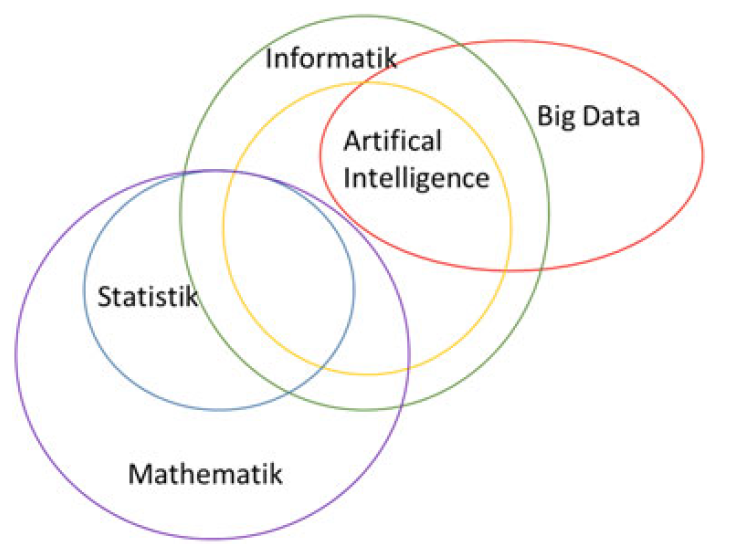
\includegraphics[width=10cm]{images/KI-Teilmengen.png}
  \caption[Teilmengen von KI]{Teilmengen von KI \cite{17}}
\end{figure}


\subsubsection{Definition und Zielsetzung}
Die Definition der künstlichen Intelligenz ist in der Literatur uneindeutig. Schon für den Begriff der Intelligenz existiert keine allgemeingültige Definition. Über die letzten Jahrzehnte hat sich sowohl der Schwerpunkt des Forschungsgebietes der KI als auch dessen Zielsetzung immer wieder gewandelt. Ihren Ursprung fand sie im Jahr 1955 mit der ersten Beschreibung durch John McCarthy \cite{11}:
\begin{quote}
  ''Ziel der KI ist es, Maschinen zu entwickeln, die sich verhalten, als verfügten sie über Intelligenz.''
\end{quote}
Mit der Schwierigkeit die Intelligenz an sich zu definieren, verliert diese Erklärung an Aussagekraft. Elaine Rich bietet im Jahr 1983 eine weitere Möglichkeit den Gegenstand der KI-Forschung zu benennen: 

\begin{quote}
''Artificial Intelligence is the study of how to make computers do things at which, at the moment, humans are better.''
\end{quote} 
Damit schafft Rich eine Beschreibung, die sowohl in der Vergangenheit als auch in der Zukunft Anwendung findet. Beispielsweise sind Menschen beim Erkennen von Objekten, Menschen oder Sprachen den Maschinen noch weit überlegen. Bild- und Spracherkennung sind wichtige Forschungsbereiche der KI. Ein zentrales Gebiet der Forschung ist demnach auch das maschinelle Lernen, denn vor allem die Lernfähigkeit des Menschen durch Adaptivität stellt sich für Computer als Herausforderung dar. Dahingegen ist die Entwicklung von Schachcomputern nicht mehr relevant, denn diese sind bereits besser als der Mensch. Dennoch geht es bei KI nicht nur um praktische Implementierungen intelligenter Verfahren. Ein Teil des Forschungsgebietes befasst sich auch mit dem Verständnis des menschlichen Handelns und Schließens (Kognitionswissenschaft). \cite{11} \newline
Das KI-System ChatGPT des Unternehmens OpenAI beschreibt künstliche Intelligenz, also seinen eigenen Hintergrund so \cite{04}:
\begin{quote}
  ''Künstliche Intelligenz (KI) ist ein interdisziplinäres Gebiet, das sich mit der Entwicklung von Algorithmen und Systemen beschäftigt, die eine menschliche Intelligenz und kognitive Fähigkeiten imitieren. KI-Systeme können Aufgaben ausführen, die normalerweise nur von Menschen erledigt werden können, wie zum Beispiel das Verstehen von Sprache, das Erkennen von Gesichtern oder das Lösen komplexer Probleme.''
\end{quote}

\begin{figure}
  \center
 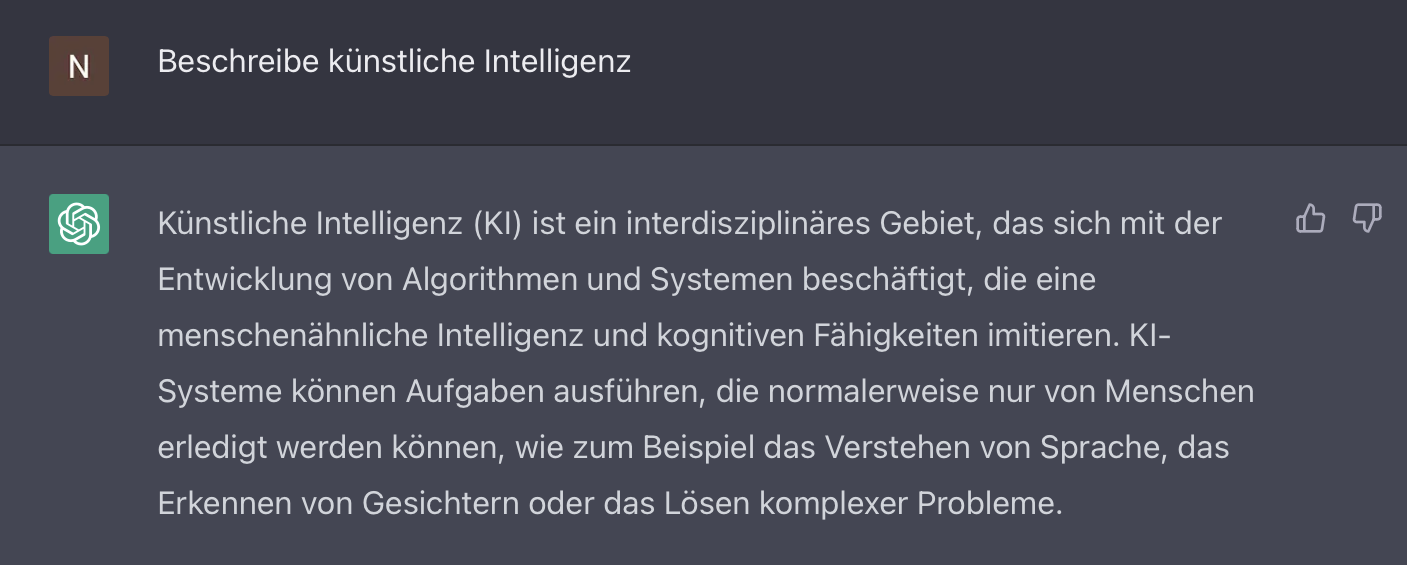
\includegraphics[width=14cm]{images/ChatGPT.png}
  \caption[KI beschrieben von ChatGPT]{KI beschrieben von ChatGPT \cite{04}}
\end{figure}
ChatGPT ist ein Chatbot, der Fragestellungen und Aufforderungen des Anwenders versteht und darauf antwortet bzw. die Aufgaben ausführt. Das Wissen ist allerdings nicht sein eigenes, denn er wurde mit großen Datenmengen trainiert, um diese Fähigkeit zu erlangen. Das beutet, dass dies nicht seine eigene Definition ist, sondern vermutlich eine Kombination aus allen Erklärungen zum Thema KI, mit dem das System trainiert wurde. Auf diesen Chatbot und die zugrundeliegende Technologie wird in einem späteren Teil der Arbeit näher eingegangen.

Der Forschungsgegenstand und die Ziele der KI haben sich seit ihren Anfängen geändert. Während früher ausschließlich an Universitäten mit Zielen wie der Entwicklung eines Schachcomputers, der dem Menschen überlegen ist, geforscht wurde, stehen heutzutage kommerzielle Anwendungen im Vordergrund. 
Gerade weil KI mittlerweile eine große Bedeutung in der Wirtschaft hat, wird mehr Geld in die Forschung investiert. So forschen nun nicht nur Universitäten, sondern auch andere Forschungsinstitute und Unternehmen in vielen Bereichen der KI. Auch die Verfügbarkeit von großen Datenmengen zu Trainingszwecken, die durch Verfahren der Daten-Analyse (Big-Data) für KI genutzt werden können, tragen einen großen Teil zu den zahlreichen Erfolgen der jüngeren Vergangenheit und Gegenwart bei. \cite{10}

\subsubsection{Turing-Test}

Im Grunde basiert künstliche Intelligenz auf statistischen Wahrscheinlichkeiten. Viele KI-Experten sehen den Begriff der KI allgemein als nichtzutreffend an. Denn derzeit handelt sich nicht etwa um Systeme, die Kreativität besitzen oder neue Ideen entwickeln. Es sind Systeme, die durch verschiedene Lernmethoden oder mit Wissen gefütterte Algorithmen, fest definierte Aufgaben erledigen. \newline
Betrachtet man nun allerdings den Turing-Test, ist der Begriff ''Intelligenz'' keineswegs falsch. Der Test wurde 1950 vom britischen Mathematiker und Informatiker Alan Mathison Turing entwickelt und ist seitdem ein überwiegend anerkannter Test, um festzustellen, ob eine Maschine intelligent ist oder nicht.
Dabei führt ein Mensch eine schriftliche Unterhaltung, ohne es zu wissen mit einer Maschine. Hier spielen weder Mimik, Gestik noch Tonalität eine Rolle. Damit die Maschine den Test besteht, müssen 30 Teilnehmer nach jeweils einem 5-minütigen Chatgespräch nicht beurteilen können, ob es sich es sich bei dem Chat-Partner um einen Menschen oder eine Maschine gehandelt hat. Die Frage nach einem Bewusstsein wird dabei nicht geprüft. Erst 2014 bestand erstmals eine Maschine den Test. \newline
Doch es gibt Kritik am Turing-Test. Davon abgesehen, dass nicht jede KI an diesem Test teilnehmen könnte, weil das Verstehen und Interpretieren von Sprache ein spezielles Feld der KI-Forschung ist, muss sich der Computer dümmer stellen als er eigentlich ist, um zu bestehen. Würde der Mensch nach der Einwohnerzahl Mannheims fragen und der Computer würde antworten ''am 31.12.2021 hatte Mannheim 311.831 Einwohner'' würde er sofort als Maschine identifiziert werden. Um den Test zu bestehen, muss sich der Computer also anpassen und taktisch verhalten. Allerdings besteht hier die Frage, ob eine solche gezielte Täuschung das Vertrauen in KI mindert.\cite{02}

\subsubsection{Schwache und starke KI}


Zur näheren Begriffsklärung wird zwischen schwacher und starker KI unterschieden. Unter schwacher KI (engl. ''Narrow AI'' oder ''Special Purpose AI'') versteht man KI-Systeme, die für einen spezifischen Zweck, bzw. zur Lösung einer fest definierten Problematik entwickelt wurden. Sie können also Aufgaben ausführen, die sonst nur Menschen bewältigen können, meistens sogar schneller und effizienter. Allerdings sind sie nicht imstande andere Aufgaben zu erledigen oder kognitive Fähigkeiten eines Menschen zu imitieren. So sind Sprachassistenten wie Siri und Alexa in der Lage Sprachbefehle zu verstehen und auszuführen, sie besitzen aber keine emotionale Kompetenz oder die Fähigkeit komplexe Probleme zu lösen. \cite{01}\cite{15}

\begin{figure}[H]
  \center
 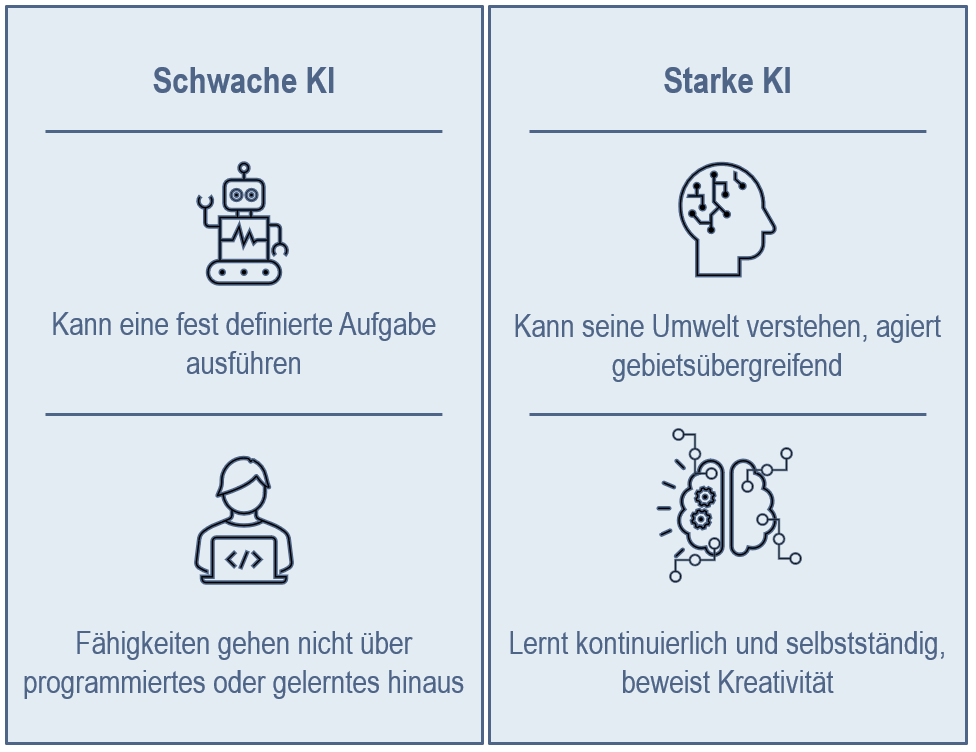
\includegraphics[width=10cm]{images/starkeschwacheKI.png}
  \caption[Schwache und Starke KI]{Schwache und starke KI (eigene Abbildung)}
\end{figure}
Im Gegensatz dazu wird bei starker KI (engl. General AI) eine komplette Nachbildung bzw. Imitation der menschlichen Intelligenz verstanden. Diese ist nicht nur auf ein Gebiet spezialisiert ist, sondern agiert gebietsübergreifend. Das bedeutet, dass sie verschiedene Aufgaben ausführen könnte, für die bisher menschliche kognitive Fähigkeiten nötig sind und dass Erkenntnisse aus einem Bereich auf andere Bereiche angewendet werden könnten. Damit wären auch für die KI unbekannte Probleme lösbar. Sie ist in der Lage ihre Umwelt zu verstehen und eigenständig zu lernen. In der aktuellen Forschung ist die Entwicklung einer starken KI jedoch nicht absehbar und wird von manchen Experten sogar als unmöglich eingestuft. Bei der Entwicklung sollten außerdem mögliche Gefahren und ethische Aspekte berücksichtigt werden. 

Im Kontext dieser Arbeit und auch in weiten Teilen der Forschung und Anwendung wird von schwacher KI gesprochen. \cite{01}\cite{15}

\subsection{Maschinelles Lernen}

Eine künstliche Intelligenz ist nicht von Beginn an intelligent. Sie muss lernen. Maschinelles Lernen (Machine Learning) ist eines der größten KI-Forschungsfelder. Anhand verschiedener Lernmethoden wird das technische System mit Daten trainiert, wodurch erst die Fähigkeiten der KI entstehen. Die jeweiligen Ansätze sind für unterschiedliche Anwendungen geeignet. \newline
Folgend werden die relevantesten Methoden genannt und kurz beschrieben. \cite{10}

\subsubsection{Supervised Learning (Überwachtes Lernen)} 

Supervised Learning ist derzeit der am weitesten verbreitete Ansatz des maschinellen Lernens. Dabei werden bekannte Daten, sogenannte Trainingsdaten genutzt. Diese enthalten bereits Ergebnisse (Label) zu den jeweiligen Eingaben. Der Algorithmus erhält zunächst nur die Eingabe und trifft eine Entscheidung über die Ausgabe. Anschließend vergleicht er seine Aussage mit dem vorgegebenen Ergebnis und passt seine nächste Beurteilung entsprechend an. Der Algorithmus wird so lange trainiert, bis nahezu immer die korrekte Entscheidung getroffen wurde. Dadurch soll der Algorithmus anschließend in der Lage sein Aussagen zu neuen, unbekannten Eingaben treffen zu können.\cite{01}\cite{05} \newline
Beispielsweise werden dem Algorithmus unsortiert Bilder von Katzen und Hunden gezeigt. Er sieht während seiner Entscheidung aber nicht das jeweilige Label "Katze'' oder "Hund". Er entscheidet anhand des Bildes, um welches der beiden Tiere es sich handelt und überprüft anschließend, ob seine Aussage korrekt war. So lernt der Algorithmus wie er Hunde und Katzen unterscheiden kann. Solche Algorithmen werden beispielsweise für Bilderkennungs-Systeme verwendet. 
\begin{figure}[H]
  \center
  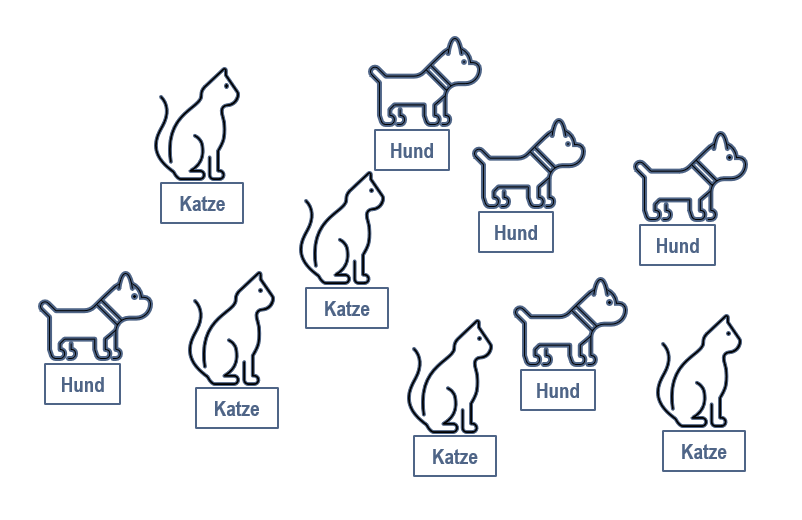
\includegraphics[width=12cm]{images/supervised.png}
  \caption[Gelabelte Bilder von Hunden und Katzen]{Gelabelte Bilder von Hunden und Katzen (eigene Darstellung)}
\end{figure}

Diese Lernmethode wird gerne genutzt, da der Entwickler hier die Kontrolle über die Trainingsdaten, also den Input hat. Es ist von Anfang an klar, welches Ergebnis am Ende stehen soll. Allerdings nimmt diese Methode viel Zeit in Anspruch, da die Daten vor der Verwendung gelabelt werden müssen. Ein Problem dieser Methodik ist auch, dass der Algorithmus nur das lernt, was er mit den Trainingsdaten beigebracht bekommt. Wird ein Algorithmus beispielsweise nur mit Bildern von schwarzen Katzen trainiert, lernt er, dass eine Katze schwarzes Fell besitzt, und wird wahrscheinlich eine weiße Katze nicht erkennen.

\subsubsection{Unsupervised Learning (Unüberwachtes Lernen)} 

Beim Unsupervised Learning versucht die KI Zusammenhänge, Ähnlichkeiten, Strukturen und Muster innerhalb einer großen Menge von Eingabedaten zu erkennen. Der Algorithmus kann so beispielsweise zur Gruppierung (Clustering) von Daten oder zur Findung von Beziehungen (Association) genutzt werden.\newline
Ein Beispiel für Clustering (K-Clustering) ist Folgendes: Dem Algorithmus werden Bilder gegeben mit der Vorgabe, dass es sich hier um zwei (K=2) Arten von Tieren handelt: Hunde und Katzen. Der Algorithmus versucht also die Bilder über mehrere Iterationen hinweg nach Hunden und Katzen zu kategorisieren. So können in der Wirtschaft Daten genutzt werden, um z.B. Personengruppen zusammenzustellen, die für eine Marketingstrategie genutzt werden können. \newline
Neben dem Clustering kann diese Lernmethode auch für sog. Associations werden genutzt, um Zusammenhänge zwischen den Daten zu finden. Eine Anwendung hierfür ist beispielsweise Amazon mit der Funktion "Kunden, die diesen Artikel gekauft haben, kauften auch diesen Artikel". \cite{01} 
\begin{figure}[H]
  \center
  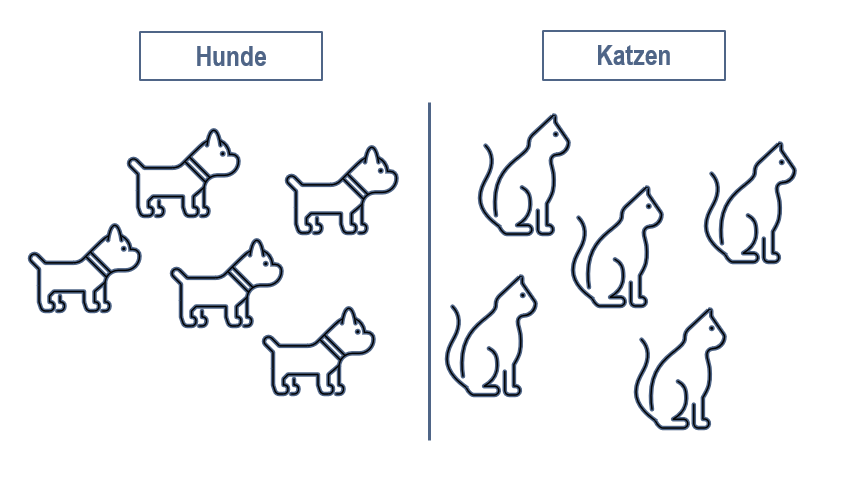
\includegraphics[width=12cm]{images/unsupervised.png}
  \caption[Clustering von Hunden und Katzen auf Grund von Eigenschaften]{Clustering von Hunden und Katzen auf Grund von Eigenschaften (eigene Darstellung)}
\end{figure}

Auch Sprachassistenten und Chatbots funktionieren mit Unsupervised Learning. Sie lernen durch die Interaktion mit Nutzern, wodurch Alexa oder Siri die Spracheingaben des Besitzers immer besser verstehen und kommunizieren können. Mit welchen Daten der Algorithmus gefüttert wird, beeinflusst also die Ausgaben der KI. Ein Beispiel für ein Problematik, die sich aus dieser Methode ergibt, war 2016 der KI-Chatbot ''Tay'' von Microsoft. Dieser hatte Zugang zu Twitter. Innerhalb von 24 Stunden entwickelten sich die zunächst einfältigen Aussagen der KI hin zu, Hetze gegen Ausländer und Feministen und der Verarbeitung von Verschwörungstheorien. Es ist allerdings nicht bekannt, ob Tay absichtlich von Nutzern mit diesen Daten gefüttert wurde.\cite{13}

\subsubsection{Reinforcement Learning (Bestärkendes Lernen)} 

Das Reinforcement Learning ist die dritte Variante Algorithmen zu trainieren. Für diese Methode werden allerdings keine Daten zum Lernen benötigt, es werden durch Ausprobieren gelabelte Daten erzeugt. \cite{17} \newline
Die Lernmethode simuliert den Lernvorgang bei Kindern. Diesen werden statt Anleitungen und Nachahmungsmuster eher Regeln beigebracht. Anschließend sollen sie dann aus eigenen Erfahrungen lernen. Mit positiver und negativer Verstärkung tritt der Lerneffekt ein. Das Kind kann dann auch zuvor unbekannte und kreative Lösungen finden.
Beim Reinforcement Learning werden also nur (Spiel-)Regeln vorgegeben. Es werden keine Lerndaten oder erwartete Ergebnisse benötigt. Durch Belohnungssignale bei richtigen Entscheidungen und Sanktionen bei falschen verbessert sich die KI in einer Simulationsumgebung anhand des Versuch-Fehler-Prinzips (Trail and Error) dann schrittweise. Das bietet nicht nur den Vorteil, dass keine großen Mengen an Lerndaten vorbereitet und zu Verfügung gestellt werden müssen, sondern auch, dass komplexe Probleme ohne menschliches Vorwissen gelöst werden können.\cite{02}
\newline
Diese Lernmethode wurde auch für die Entwicklung der Spielsoftware AlphaGo Zero verwendet. Nur mit der Kenntnis der Spielregeln und durch Spielen gegen sich selbst, gelang es dem Computer eine große Spielstärke zu entwickeln. Außerdem nutzte er bislang unbekannte Spielzüge und -varianten. Mögliche Belohnungssignale für AlphaGo Zero wären z.B. ''Spiel gewonnen" oder ''möglichst große Anzahl verbleibender eigener Spielsteine am Ende der Partie''.
\cite{02}

\subsection{Künstliche Neuronale Netze}

Die wohl bekannteste Technologie der KI-Forschung sind Künstliche Neuronale Netze, kurz KNN (engl. Artificial Neural Network, ANN). Sie sind ein Teil des maschinellen Lernens und sind angelehnt an eine natürliche Vernetzung von Neuronen in einem Nervensystem eines Lebewesens. Dabei geht es weniger um die biologische Nachbildung, sondern mehr um eine Abstraktion von Informationsverarbeitung. \cite{17}

\begin{figure}[H]
  \center
 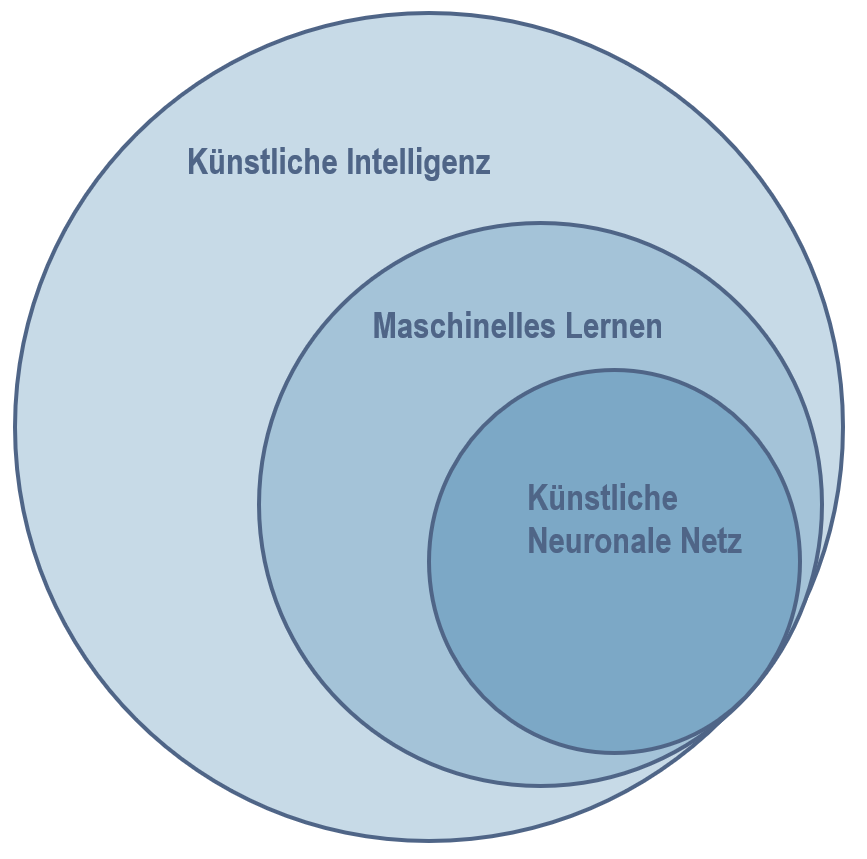
\includegraphics[width=7cm]{images/EinordnungKNN.pptx.png}
  \caption[Neuronale Netze als Teilmenge von KI]{Neuronale Netze als Teilmenge von KI (eigene Abbildung nach \cite{17})}
\end{figure}

Bei Künstlichen Neuronalen Netzen sind die Neuronen in sog. Schichten (engl. Layers) angeordnet. Der Begriff ''Topologie'' beschreibt dabei wie viele künstliche Neuronen sich auf wie vielen Schichten des KNN befinden und wie diese miteinander über sogenannte Kanten verbunden sind. Ein einfaches neuronales Netz besteht aus einer Eingabeschicht (input layer), einer verdeckten Schicht (engl. hidden layer), und einer Ausgabeschicht (output layer). Die verdeckte Schicht kann dabei beliebig breit sein, d.h. es können beliebig viele Neuronen nebeneinander in dieser Schicht angeordnet sein. Sobald sich in einem KNN mehr als eine verdeckte Schicht befindet, wird von einem Tiefen Neuronalen Netz gesprochen. Da es sich bei einem KNN selten um einschichtige Netzwerke handelt, wird im Sprachgebrauch meistens unabhängig von der Tiefe von neuronalen Netzen gesprochen. \cite{17}

\begin{figure}[H]
  \center
 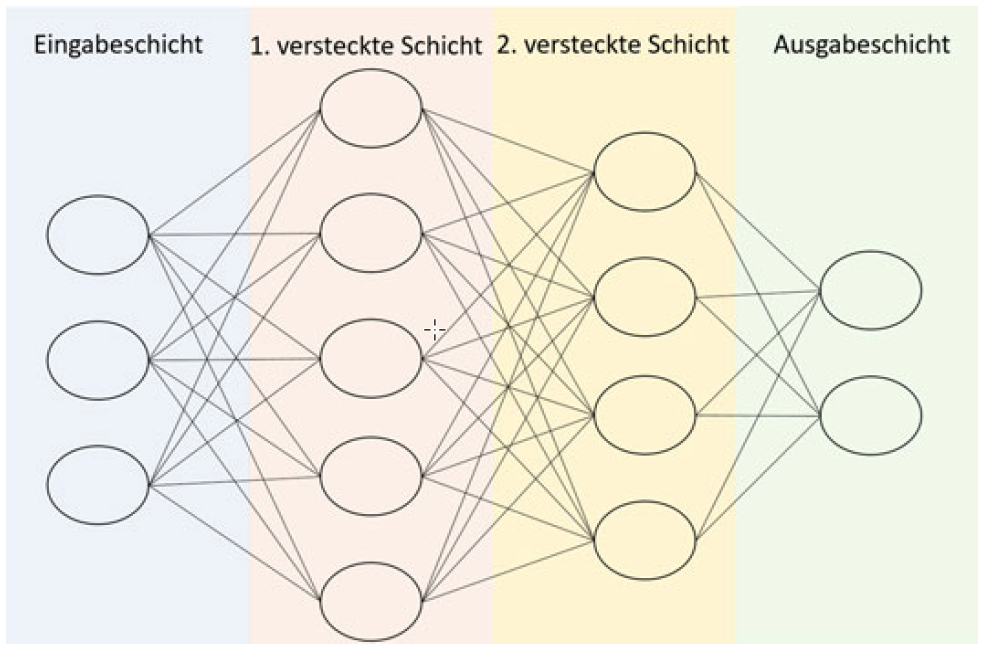
\includegraphics[width=11cm]{images/KNN-Schichten.png}
  \caption[Aufbau eines neuronalen Netzes]{Aufbau eines neuronalen Netzes \cite{17}}
\end{figure}

Die Neuronen bekommen jeweils Eingaben von den Neuronen der vorherigen Schicht und geben dann eine gewichtete Ausgabe an die nächste Schicht weiter. Je mehr Gewicht eine Verbindung zwischen Neuronen enthält, desto intensiver ist hier der Informationsfluss. Dieses Prinzip wird als Deep Learning bezeichnet und stellt heutzutage den Standard-Anwendungsfall von neuronalen Netzen dar. Deep Learning wird in den Bereichen des maschinellen Lernens angewendet und würde sich in Abbildung 2.6 als Teilmenge dieses Gebietes wiederfinden. Dabei werden wie im menschlichen Hirn die Verbindungen zwischen den Neuronen je nach Gelerntem entweder gestärkt oder geschwächt. So werden über viele verdeckte Schichten und Lerniterationen hinweg komplexe Datenzusammenhänge entwickelt.\newline
Durch verschiedene Arten von neuronalen Netzen können verschiedene Probleme gelöst werden. So werden beispielsweise Konvolutionale Neuronale Netze (CNNs) für die Verarbeitung von Bildern und Videos verwendet und Generative Adversarial Networks (GANs) zur Generierung von authentischen künstlichen Daten, wie künstliche Bilder oder Stimmen. Dies sind nur zwei Beispiele von Vielen.\cite{17} 

Problematisch ist das sog. ''Black Box''-Verhalten. Die verdeckten Schichten tragen diesen Namen, weil man nicht nachvollziehen kann, was wirklich in ihnen passiert. Der Mensch kann also nicht erkennen, warum die KI am Ende die jeweilige Entscheidung getroffen hat. Ein Beispiel für diese Problematik beschreibt Prof. Ulrich Walter von der TU München bei einem Vortrag über künstliche Intelligenz im deutschen Museum am 19.10.2022: Eine KI wurde durch Deep Learning darauf trainiert Schiffe zu erkennen. Dies hat das System auch sehr gut geschafft. Bei Betrachtung der sog. Heat-Map, die anzeigt aus welchen Bereichen der Bilder die KI schließen konnte, dass es sich um ein Schiff handelt, wurde klar, dass sie nicht das Schiff, sondern das Wasser erkannte. Daraus lässt sich schließen, dass der Algorithmus nur mit Bildern von Schiffen auf dem Wasser trainiert wurde. Sie erkennt also das Wasser als ''Schiff''.\cite{16}

\begin{figure}[H]
  \center
 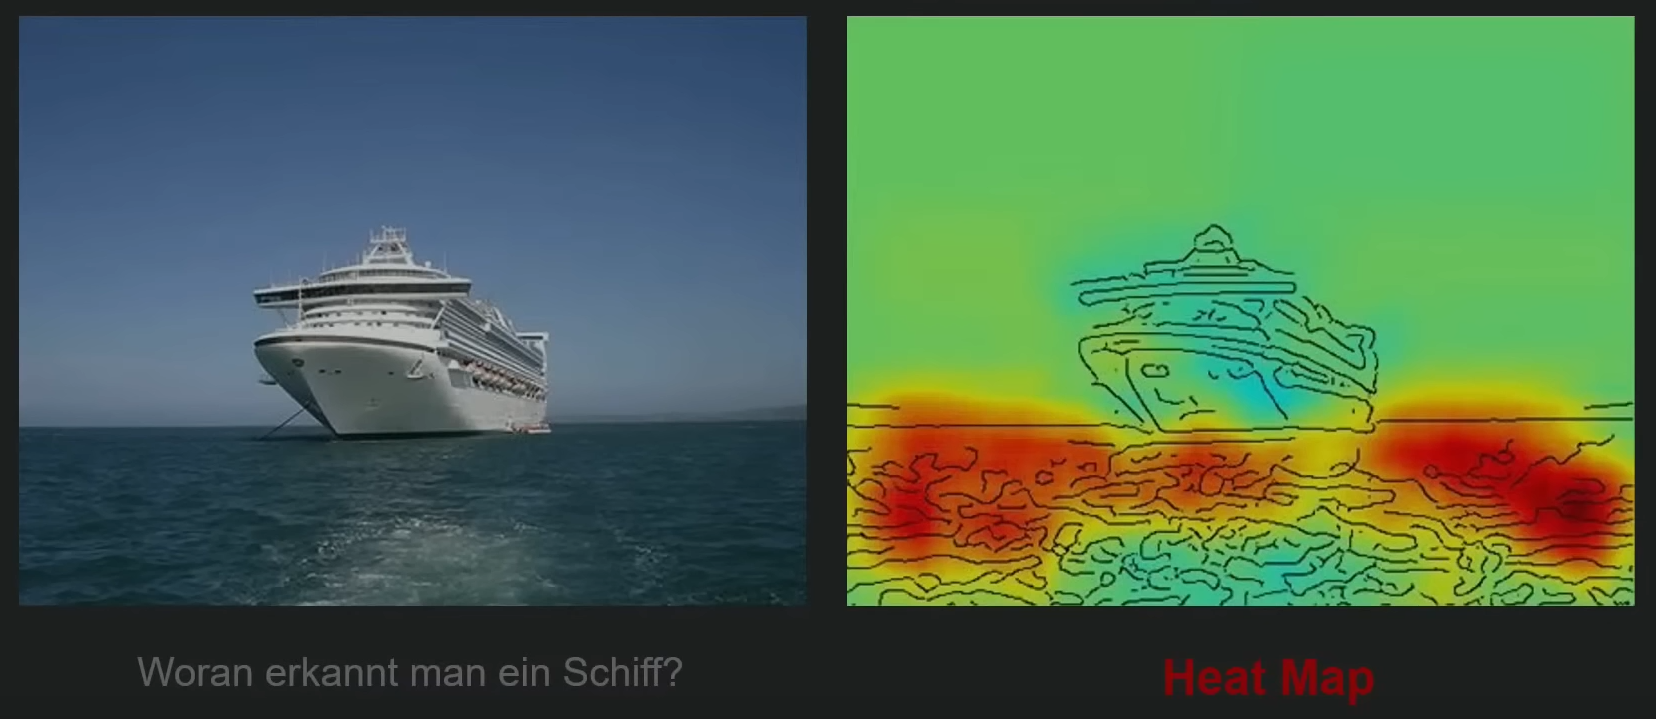
\includegraphics[width=14cm]{images/Schiff-HeatMap.png}
  \caption[Heat Map zur Erkennung eines Schiffes]{Heat Map zur Erkennung eines Schiffes (Übernommen aus Vortrag \cite{16})}
\end{figure}

Ähnliches ist auch beim Trainieren einer KI auf die Erkennung von Pferden in Bildern passiert. Hier wurde der Algorithmus wohl überwiegend mit Bildern trainiert, die Worte wie ''Pferd'' beinhalteten. \cite{16}

\begin{figure}[H]
  \center
 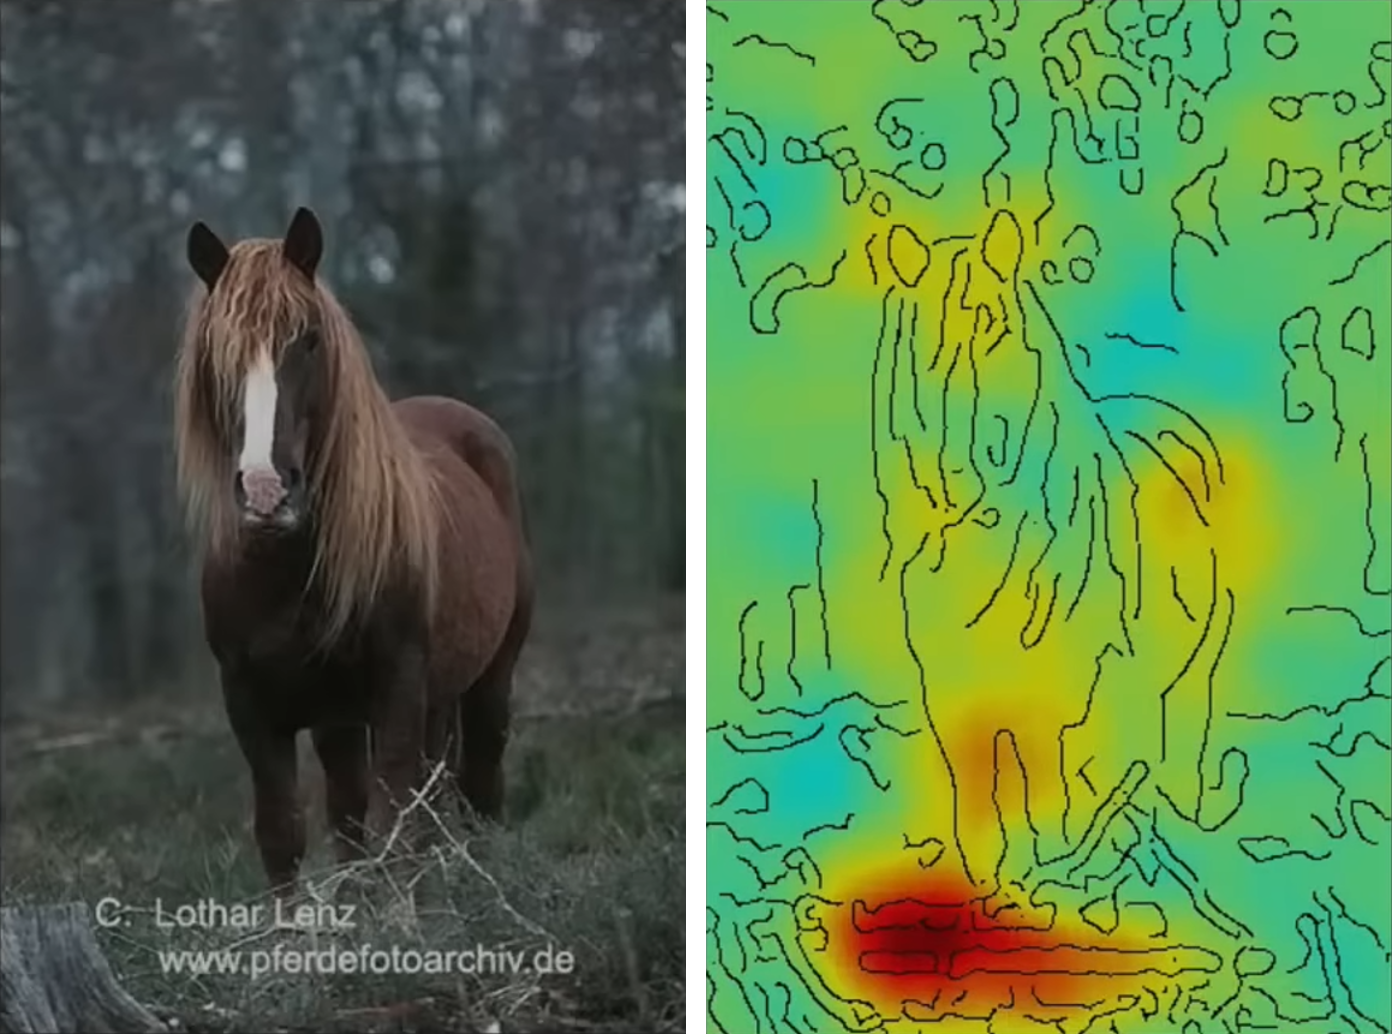
\includegraphics[width=10cm]{images/Pferd-HeatMap.png}
  \caption[Heat Map zur Erkennung eines Pferdes]{Heat Map zur Erkennung eines Pferdes(Übernommen aus Vortrag \cite{16})}
\end{figure}

Zusammenfassend lässt sich sagen, dass neuronale Netze bzw. Deep-Learning-Netze in den letzten Jahren Durchbrüche in zahlreihe Bereichen erzielt haben. Darunter zählt das Treffen von Voraussagen, das automatische Erkennen von Objekten auf Bildern und das Verstehen und Verfassen von Texten. Die Qualität eines neuronalen Netzes hängt dabei stark von den verwendeten Lerndaten, bzw. den vorgegebenen Regeln (bei Reinforcement Learning) ab. 

\subsection{Weitere Technologien und Anwendungen}

\subsubsection{Regelbasierte und Experten-Systeme}

Neben den lernenden KI-Systemen, die mit großen Mengen an Daten trainiert werden, gibt es auch regelbasierte Systeme. Der Mensch gibt hier einfach gesagt durch If-Then-Beziehungen oder einen Entscheidungsbaum feste Regeln vor anhand das Systeme Entscheidungen treffen soll. Eines dieser Systeme ist das sog. Expertensystem. Der Experte gibt dem Algorithmus sein Expertenwissen über die spezielle Aufgabe bzw. die Problematik. Das System kann dann anhand von Kriterien, die er nicht selbst gelernt hat, sondern die ihm vorgegeben wurden, automatisiert Entscheidungen treffen. Diese Systeme sind in der Regel leichter zu implementieren, sie werden allerdings schnell sehr komplex und unübersichtlich.\cite{01}
Anwendung findet regelbasierte KI-Systeme vor allem in Bereichen, in denen ein hohes Maß an Zuverlässigkeit und Sicherheit erforderlich ist und Entscheidungen des Systems einfach vom Experten überprüfbar sind. 
Ein Anwendungsbeispiel wäre ein medizinisches Diagnose-System, das anhand von Untersuchungsresultaten und Symptomen bestimmte Krankheiten diagnostiziert.

\subsubsection{Computer Vision} 

Der Forschungsbereich Computer Vision (computerbasiertes Sehen) beschäftigt sich mit der Verarbeitung und Analyse von visuellen Daten, sowohl Bilder als auch Videos. Ziel ist es, dass der Computer die Inhalte des Bildes erkennt und versteht. Im industriellen Umfeld werden oft auch von Machine Vision (Maschinelles Sehen) gesprochen. 
Durch spezielle Algorithmen und mathematische Modelle versucht der Computer einem Bild geometrische Formen, Kanten und zusammenhängende Bildbereiche zu identifizieren. In einem nächsten Schritt können so auch ganze Objekte erkannt werden. 
Computer Vision findet Anwendung beispielsweise im Erkennen von Gesichtern, Identifizierung von kranken Geweben, oder auch beim autonomen Fahren. Aber auch im klassischen industriellen Umfeld ist Computer Vision eine weit verbreitete Technologie.


\subsubsection{Natürliche Sprachverarbeitung}  
 
Ein weiterer Bereich der KI-Forschung ist die natürliche Sprachverarbeitung (engl. Natural Language Processing, NLP) oder auch Computerlinguistik (CL). Anstatt wie bei Computer Vision Bilder oder Videos zu verarbeiten, fokussiert sich NLP auf das Erkennen und Verstehen von Sprache und Texten. Verwendete Daten werden sowohl in schriftlicher Form als auch als Audio-Dateien verwendet. Der Bereich gliedert sich in die zwei Bereiche Natural Language Unterstanding (NLU), also das Verstehen von Sprache und Natural Language Generation (NLG), dem Generieren von Sprache. \newline
Anwendungen von NLP sind beispielsweise Text-to-Speech- und Speech-to-Text-Systeme, maschinelle Übersetzung von Sprache, Sprach- bzw. Stimmerkennung und Textgenerierung. 
Der ChatBot ChatGPT ist ebenfalls eine Anwendung dieses Forschungsbereichs. GPT steht dabei für Generative Pre-training Transformer, wobei Transformer für eine spezielle Art von neuronalem Netzwerk ist, welches für die verbesserte Verarbeitung von natürlicher Sprache entwickelt wurde. GPT wurde mit großen Mengen an Texten trainiert und hat durch eine Vielzahl nach Kenntnissen und Fähigkeit erworben. Es kann auf Fragen antworten, Texte generieren und weitere Aufgaben ausführen.\cite{04} 
Allerdings muss beachtet werden, dass diese Technologie nur so schlau ist, wie die Daten, mit welchen sie trainiert wurde. Beispielsweise kann ChatGPT die Frage ''Wer wurde 2022 Fußballweltmeister?'' nicht beantworten. 

\begin{figure}[H]
  \center
 \includegraphics[width=10cm]{images/Faußballweltmeister.png}
  \caption[Screenshot ChatGPT]{Screenshot ChatGPT}
\end{figure}

In diesem Beispiel sagt ChatGPT, dass er die Antwort nicht weiß. doch in anderen Fällen ist sein Unwissen weder zu erkennen, noch sagt er, dass er sich bei der Antwort nicht sicher ist. Bei der Frage nach Medizintechnik-Firmen in Augsburg listet werden fünf Firmen aufgelistet, wobei keine davon wirklich in Augsburg existiert.

\subsubsection{Robotik} 

Wenn in den Medien von künstlicher Intelligenz die Rede ist, werden häufig Roboter gezeigt. Allerdings ist KI nur ein Teil der Robotik. Trotzdem stellt große Teile der Robotik Untergebiete der KI-Forschung dar. Außerdem hat die Robotik und vor allem als Teil der KI einen hohen Stellenwert in der heutigen Industrie.
Roboter bestehen zu großen Teilen aus Hardware, wie mechatronische Komponenten, Sensoren und Aktoren. Sie sind nicht per se lernfähig oder besitzen künstliche Intelligenz. Roboter sind programmierbare Maschinen, die selbstständig definierte Aufgaben verrichten. Die Unterscheidung zu Computern und anderen Maschinen ist die frei beweglichen Achsen, wodurch der Roboter die Fähigkeit bekommt Bewegungen auszuführen. Dabei gibt es einfache Verrichtungsroboter und welche, die zusätzlich mit künstlicher Intelligenz ausgestattet sind. 
Eine KI-Technologien die häufig in der Robotik verwendet wird, ist Computer Vision. So kann der Roboter seine Umwelt bzw. seinen Arbeitsbereich wahrnehmen und auf Grundlage dessen Entscheidungen treffen. Ein Beispiel wäre ein Greifarm, der ein Bauteil abhängig von dessen aktuellen Lage greifen kann, um es dann durch Rotation an der vorgesehenen Stelle anzubringen.
Allgemein werden Roboter in Kombination mit KI in automatisierte Fabriken, der Medizin, aber auch in der Pflege und Bildung eingesetzt. \cite{19}

\section{Produktion}

Die Produktion ist eine der Grundfunktionen eines Unternehmens und ist verantwortlich für die Leistungserstellung. Sie hat einen großen Einfluss auf die Wirtschaftlichkeit. In diesem Abschnitt der Arbeit wird der Unternehmensbereich der Produktion näher beleuchtet.

\subsection{Grundlagen und Ziele der Produktion}

Erich Gutenberg (1897-1984) gilt in Deutschland als Gründer der modernen Betriebswirtschaftslehre gilt. Er definierte die Produktion in Band 1 seiner Buchreihe \textit{Grundlagen der Betriebswirtschaftslehre} wie folgt:

\begin{quote}
 ''Eine Leistungserstellung, die außer Arbeitsleistungen und Betriebsmitteln auch den Faktor Werkstoffe enthält, bezeichnen wir als 'Produktion'.'' \cite{20}
\end{quote}

Damit beschreibt er die Produktionsfaktoren in der Betriebswirtschaftslehre: menschliche Arbeit (inklusive Faktoren wie Arbeitsbedingungen oder -entgelt), Betriebsmittel (z.B. Maschinen, Werkzeuge und Gebäude) und Werkstoffe (Rohstoffe, Hilfsstoffe und Betriebsstoffe). Diese werden auch als Elementarfaktoren bezeichnet. Dispositive Faktoren sind hingegen beispielsweise die Betriebsführung und das Wissen im Unternehmen. Generell umfasst der Begriff der Produktionsfaktoren alles was zur Leistungserstellung und zur Aufrechterhaltung und Ausbau der Leistungsbereitschaft dient. \cite{06}

\begin{figure}%[H]
  \center
  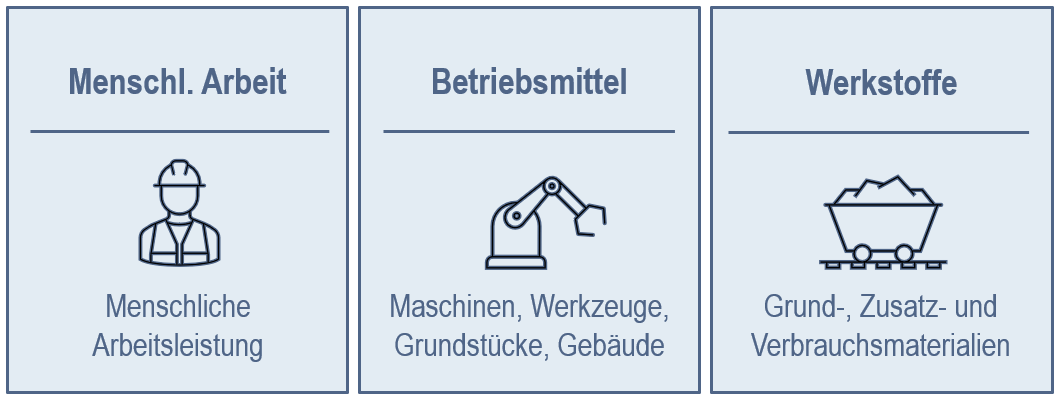
\includegraphics[width=12cm]{images/Elementarfaktoren.pptx.png}
  \caption[Elementarfaktoren]{Elementarfaktoren (eigene Darstellung)}
\end{figure}

\begin{figure}%[H]
  \center
  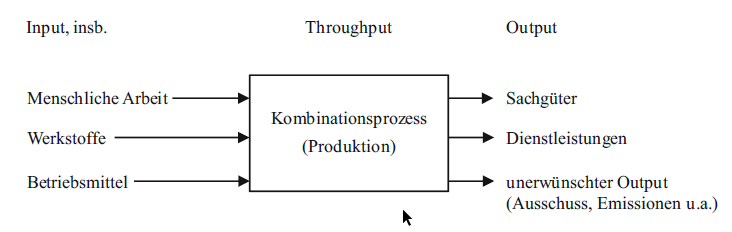
\includegraphics[width=12cm]{images/Kombinationsprozess.png}
  \caption[Kombinationsprozess der Produktion]{Kombinationsprozess der Produktion (übernommen von \cite{07}) }
\end{figure}

Durch den gelenkten Einsatz der Produktionsfaktoren werden also Güter oder Dienstleistungen hergestellt. Diese sind je nach Fertigungsgrade beispielsweise Halbfabrikate, Zwischenprodukte oder Endprodukte.\cite{12}
Die Produktion lässt sich durch die sog. Produktionsfunktion als funktionalen Zusammenhang zwischen der Ausbringungsmenge (engl. Output) und der eingesetzten Produktionsfaktoren (engl. Input) bei gleichbleibender Produktionstechnologie beschreiben. \cite{20}

\begin{equation}
  x = f(r_1,r_2,...r_n) 
\end{equation}
x: Ausbringungsmenge des Produktes \\
$r_{i}$: Einsatzmenge des Produktionsfaktors i \\

% Kostenfunktion


In der Wirtschaft lassen sich Ziele unter anderem in ökonomische (Gewinn, Kosten, Wirtschaftlichkeit) und nicht ökonomische Ziele (Menge, Qualität der Produkte, Termineinhaltung) unterteilen. Auf beide Zielarten hat die Produktion einen großen Einfluss oder sind maßgeblich an der Erreichung beteiligt.

Durch die Nutzung von nicht-ökonomischen Kennzahlen wie der Auslastung, der Produktivität und der Effektivität lässt sich die Leistungsfähigkeit eines Produktionsprozesses beurteilen. Sie setzen mengenmäßige Größen (Output und Input) in Verhältnis und orientieren sich dabei am ökonomischen Prinzip. Dieses beinhaltet das Maximal- und das Minimalprinzip, wobei das Maximalprinzip die Erreichung des maximalen Outputs bei gleichbleibendem Input beschreibt und das Minimalprinzip einen möglich minimalen Input für einen gleichbleibenden Output. 

Die Auslastung bezieht sich auf den Input des Produktionsprozesses und setzt den tatsächlichen Input an Produktionsfaktoren mit der geplanten Input-Menge in Beziehung. Sie beschreibt ''wie viel gearbeitet'' wird. \cite{20}

\begin{equation}
  Auslastung =\frac{Ist-Input}{Plan-Input}
\end{equation}

Die Produktivität oder auch Effizienz beschreibt das Verhältnis vom mengenmäßigen Output zum Input und ermittelt so die Ergiebigkeit der Produktion. Hiermit kann entweder der gesamte Prozess beurteilt, aber auch faktorspezifische Aussagen getroffen werden. Hierfür wird die gesamten Ausbringungsmenge mit der Einsatzmenge eines Faktors in die Formel eingesetzt. \cite{20}

\begin{equation}
  Produktivit"at =\frac{Ist-Output}{Ist-Input}
\end{equation}

Inwieweit das Produktionsergebnis der Planung entspricht, wird durch die Effektivität ermittelt. Diese Kennzahl kann sich sowohl auf die Menge als auch auf die Dauer des Prozesses oder die Qualität des Produktes oder der Dienstleistung beziehen. Hier werden also der Ist-Output mir dem planmäßigen Output ins Verhältnis gesetzt.\cite{20}

\begin{equation}
 Effektivit"at =\frac{Ist-Output}{Plan-Output}
\end{equation}


Neben diesen nicht-ökonomischen, technisch-orientierten Kennzahlen werden auch ökonomische Zielgrößen, wie die Wirtschaftlichkeit für die Beurteilung der Produktion verwendet. Sie misst das Verhältnis zwischen monetären Größen, also zwischen dem wertemäßigen Output (z.B. Ertrag, Erlöse, Einzahlungen) und dem wertemäßigen Input (z.B. Aufwand, Kosten, Auszahlungen).\cite{7}

\begin{equation}
  Wirtschaftlichkeit =\frac{wertem"aßiger Output}{wertem"aßiger Input}
\end{equation}

Bei Betrachtung der dieser Kennzahlen, könnten sich beispielsweise folgende Ziele ergeben, die jeweils von verschiedenen Bereichen der Produktion abhängen: hoher Output, hohe Produktqualität, Termineinhaltung, Auslastung der Maschinen und Fertigungsbereiche, geringe Durchlaufzeit. 

\subsection{Produktionsaufbau und -ablauf}
Es gibt vielen Arten eine Produktion zu klassifizieren. Denn mit der Vielfalt an Produkten auf dem Markt steigt auch die Vielfalt der Fertigungsprozesse. Abhängig vom Produkt lassen sich bereits mindestens fünf Merkmale unterscheiden: nach Güterart, Gestalt, Zusammensetzung, Beweglichkeit der Güter und Spezifizierung des Produktes. Anhand dieser Merkmale kann dann auch auf Programmeigenschaften geschlossen werden, durch die Unterscheidung der Anzahl der Produktarten, des Leistungstypen der Produktion und der Beziehung des Produktes zum Absatzmarkt.\cite{07} In den folgenden beiden Abbildungen sind die Ausprägungen der Produktions- und Programmmerkmale zusammengefasst. Handelt es sich bei dem Produkt beispielsweise um eine Zahnbürste, würde diese wie folgt eingeordnet werden:
\begin{figure}[H]
  \center
 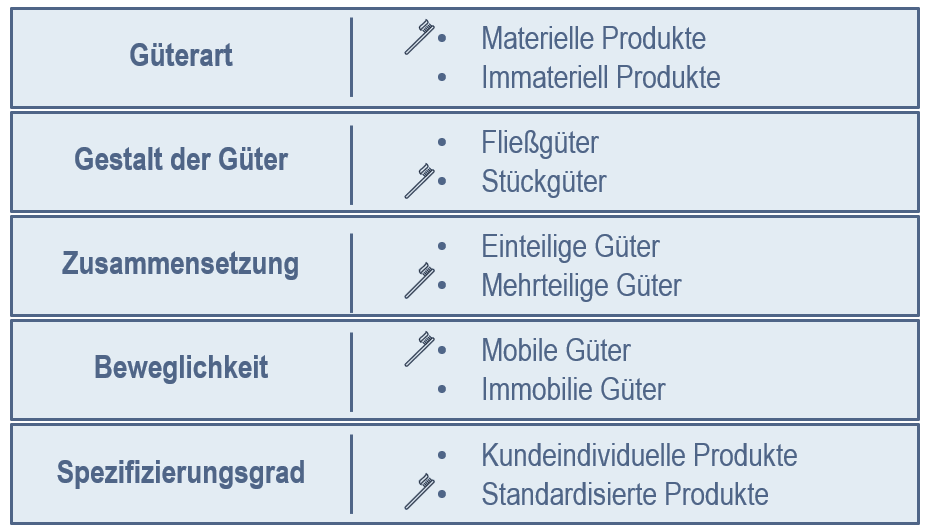
\includegraphics[width=10cm]{images/nachProdukt.pptx.png}
  \caption[Produktionstypen nach Produkteigenschaften]{Produktionstypen nach Produkteigenschaften (leicht verändert übernommen von \cite{07})}
\end{figure}
\begin{figure}[H]
  \center
 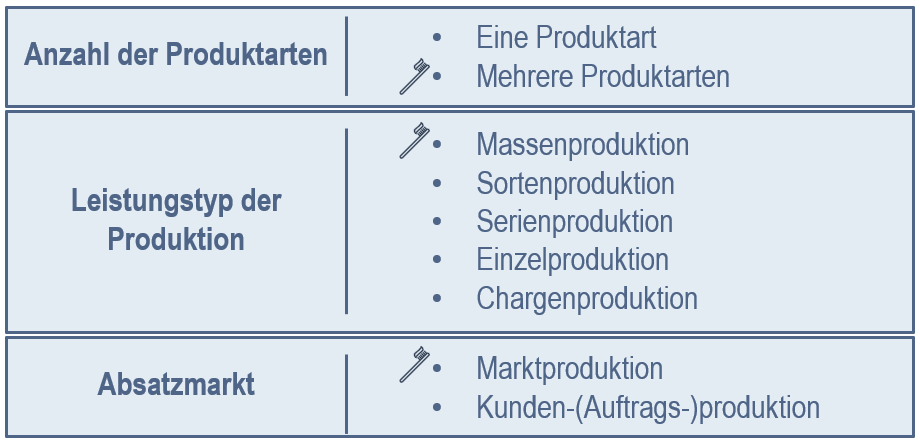
\includegraphics[width=10cm]{images/nachProgramm.png}
  \caption[Produktionstypen nach Programmeigenschaften]{Produktionstypen nach Programmeigenschaften (leicht verändert übernommen von \cite{07})}
\end{figure}

Diese Klassifizierung eines Produktes hilft dabei den Produktionsaufbau und -ablauf zu planen. Hinzu kommt noch die Bestimmung der Fertigungsverfahren, wobei diese Unterteilung nicht weiter in dieser Arbeit behandelt wird. Ja nach Fertigungsverfahren ergeben sich Produktionsabläufe mit (auch abhängig vom Fabriklayout) gegebenenfalls Umrüstvorgänge, Lager- bzw. Wartezeiten, Transportwege, Reihenfolge der Fertigungsschritte und weiteren Besonderheiten. Ist diese Planung einmal umgesetzt, ist es aufwändig und kostenintensiv Änderungen im Aufbau und Ablauf zu implementieren, weshalb dies einen wichtigen Teil einer Produktion darstellt. \cite{07}

\subsection{Produktionsprogramm}

Steht die Fertigung, geht es mit der operativen Planung weiter. Für Produktionsplanung und -steuerung wird ein Produktionsprogramm erstellt. Inhalt des Programms ist neben einer Übersicht über die Produkte und die jeweilige Menge die innerhalb eines bestimmten Zeitraums produziert werden soll auch die Ressourcen die dafür notwendig sind, wie Materialien, Maschinen und Arbeitskräfte. Außerdem wir durch ein Produktionsprogramm sichergestellt, dass die benötigte Menge an Produkten oder Dienstleistungen produziert werden, um die Kundenachfrage zu befriedigen. Auch Überstunden, Engpässe und Überproduktion kann durch ein gutes Produktionsprogramm vermieden werden. Zur Erstellung werden Informationen wie Verkaufsprognosen und Saisonalitäten berücksichtigt. Das Programm sollte an veränderte Bedingungen, wie z.B. Lieferengpässe, Änderung der Kundennachfrage oder technischen Fortschritt angepasst werden. Um einen reibungslosen Ablauf der Produktion zu unterstützen sollte das Produktionsprogramm sorgfältig und geplant und auch überwacht werden. \cite{07}
%strategische, taktische, operative Produktionsprogrammplanung 07 S.107

\subsection{Kontrolle und Überwachung der Produktion}

Zur Überwachung und Kontrolle der Produktion zählt vor allem das Qualitätsmanagement (kurz QM). Das QM hat generell das Ziel zu vermeiden, dass fehlerhafte Produkte den Kunden erreichen, oder Maßnahmen zu ergreifen, wenn dies doch passiert. Dazu werden statistische Methoden wie die Stichprobe genutzt, um an verschiedenen Stellen der Produktion von einzelnen Gütern auf die Qualität der gesamten Serie schließen zu können. Übersteigt die Anzahl an fehlerhaften Teilen einen festgelegten Grenzwert, wird dieser Fehler analysiert und der Versuch unternommen die Ursache zu finden und zu beheben. \cite{07}

Neben der Qualität wird auch die Leistung einer Produktionsanlage Überwacht. Dabei wird der Ist-Output mit dem Plan-Out verglichen. Die Leistung sagt also etwas über die Effektivität einer Produktion aus und kann sich auf verschiedene Sachen beziehen, wie z.B. auf die Zeit, die Anzahl der Produkte oder die Qualität. Weicht Leistung vom Sollwert zu weit ab, muss die Ursache identifiziert und Maßnahmen ergriffen werden. \cite{07}

Die Wartung der Produktionsanlagen kann auch als Teil der Überwachung der Produktion gesehen werden. Dabei werden die Anlagen auf ihre Funktionstüchtigkeit überprüft und Maßnahmen zur Erhaltung dieser getroffen, wie z.B. das Nachfüllen von Schmierstoffen. Durch die Wartung der Maschinen können Qualitäts- und Leistungsmängel vermieden werden, sie kann aber auch eine Maßnahmen zur Behebung dieser Mängel sein. Werden Wartungen nicht regelmäßig durchgeführt, kann dies zu Schäden an den Anlagen und Produkten und auch Komplettausfällen führen. Dadurch entstehen meist hohe Kosten, die Wartung und Prüfung der Produktionsanlagen zu einem wichtigen Teil der Produktion machen. \cite{07}

% \subsection{Herausforderungen und Schwierigkeiten}

% In der Produktion kommen viele Faktoren zusammen. Sowohl interne Bereiche des Unternehmens, wie Einkauf, Vertrieb und Management haben einen Einfluss auf den Erfolg der Produktionen, als auch externe Faktoren wie Lieferanten, Rohstoffpreise und die politische Lage.
% Probleme und Herausforderungen können also aus unterschiedlichem Ursprung stammen und sind oft nicht beeinflussbar. Mit einer guten Produktionsplanung können allerdings mögliche Risiken berücksichtigt und auftauchende Schwierigkeit gelindert oder vermieden werden.

% Viele Herausforderungen und Probleme, die in der Produktion selbst auftreten, können beispielsweise mit dem Einsatz von Technologien, wie künstlicher Intelligenz 

% Engpässe, Lieferschwierigkeiten, Qualitätsprobleme, Kostenprobleme

\chapter{Künstliche Intelligenz in der Produktion}
Die Herausforderungen, die eine Produktion, deren Planung, Durchführung und Überwachung mit sich bringt, können durch neue Technologien besser gemeistert werden. Deshalb spielen in modernen produzierenden Unternehmen Themen wie ''Smart Factory'', ''Internet of Things (IoT)" und ''Manufacturing 4.0" ein große Rolle. Sie versprechen eine Steigerung der Produktivität, weniger Überproduktion, bessere Vorhersagen und automatisierte Fertigungsprozesse. Sie stehen unter dem großen Überbegriff der Digitalisierung und Industrie 4.0. Doch welche Rolle künstliche Intelligenz aktuell in der Produktion spielt wird in diesem Kapitel behandelt.

\section{Einordnung von KI in Industrie 4.0}
Der Begriff Industrie 4.0 beschreibt die umfassende Digitalisierung der industriellen Produktion und wurde ursprünglich als Name für ein Zukunftsprojekt der deutschen Bundesregierung. Ziel ist eine weitestgehend selbstorganisierte Produktion in der Menschen, Maschinen, Produkte und Logistik untereinander kommunizieren und kooperieren können. Der Begriff soll eine Anspielung auf eine vierte industrielle Revolution sein und diese selbst einleiten. IT soll mit Produktionstechnologien verschmelzen, wodurch sich für die produzierenden Unternehmen viele Potentiale erschließen. \cite{22}Vor allem in der Fertigung sehen die Unternehmen laut einer Studie von Deloitte aus dem Jahr 2018 das größte Anwendungsgebiet von Industrie 4.0 Technologien.\cite{23}

%Abbildung Deloitte

Doch in der Realität sieht heutzutage noch anders aus. Laut der Deloitte-Studie werden eher einzelne Technologien verwendet, um einen Bereich effizienter zu gestalten, produktionsübergreifende ganzheitliche Lösungen, wodurch die Einzelanwendungen sich gegenseitig verstärken würden sind eher die Seltenheit.

Auch Technologien der künstlichen Intelligenz spielen in der Industrie 4.0 eine Rolle. Doch erst eine fortschreitender Digitalisierung ermöglicht den Einsatz. Für die meisten Anwendungen vor allem aus dem Bereich des maschinellen Lernens sind große Datenmengen erforderlich. Diese existieren zwar, sind jedoch auf verschiedene Systeme verteilt und können nur schwer zusammengebracht werden. Doch auch schon heutzutage gibt es Beispiele von Produktionen in welchen KI-Systeme erfolgreich zum Einsatz kommen. Im Jahr 2020 befragte Bitkom Industrieunternehmen verschiedener Größen (am 100 Mitarbeiter), ob sie Künstliche Intelligenz im Kontext von Industrie 4.0 im Unternehmen nutzten. Nur etwa 10\% der Unternehmen mit 100 bis 500 Mitarbeiter beantworteten diese Frage mit ''ja'', bei größeren Unternehmen (ab 500 Mitarbeiter) waren es knapp jeden Vierte.\cite{27} 
 
\section{Anwendungen in der Produktion}
Das Frauenhofer Institut sieht in einer Studie acht Anwendungsfelder von KI für produzierenden Unternehmen in produktionsnahen Bereichen: Instandhaltung, Logistik, Qualitätsmanagement und -kontrolle, Produkt- und Prozessentwicklung, Digitale Assistenzsysteme, Prozessoptimierung und -steuerung, Ressourcenplanung, und Automatisierungstechnik.\cite{24} Fünf dieser Bereiche werden in diesem Abschnitt der Arbeit mit konkreten Anwendungsbeispielen näher beschrieben.

\subsubsection{Instandhaltung}
Ohne Einsatz von KI in der Instandhaltung wird Maschinen in regelmäßigen Intervallen gewartet. Da es dann keine Informationen über den Zustand der Maschinen zwischen den Wartungen gibt, müssen die Intervalle so kurz sein, dass Ausfälle oder Schäden vermieden werden können. Durch KI-Anwendungen können die Wartungsintervalle bedarfsgerecht optimiert werden. Bei der vorbeugenden Wartung überwacht die KI Maschinen- und Prozesskenngrößen um die Abnutzung des Betriebsmittels zu ermitteln und entsprechend einen Wartungsbedarf einzelner Komponenten zu signalisieren. Dadurch wird die Terminierung der Wartungen zunehmend automatisiert und ermöglicht die Fokussierung auf einzelne Komponenten, anstatt einer Komplettwartung. Dies kann mit Hilfe von Aktionsplan-Algorithmen verwirklicht werden. Diese werden auf entsprechende Daten und Entscheidungen aus früheren Szenarien trainiert. Auch Anwendungen aus der Bild und Tonverarbeitung können für diese Art von Wartung genutzt werden. Durch Erweiterung der vorbeugenden Wartung durch weitere Algorithmen oder maschinelles lernen können vorhersagende Wartungssystemen (engl. Predictive Maintenance)  entwickelt werden. Hiermit ist eine Vorhersage über potentielle Ausfälle von Komponenten möglich anhand von Trendanalysen und komplexer Mustererkennung. \cite{24}

Die häufigste Anwendung von KI in der Instandhaltung war 2019 bei über 300 befragten deutschen Firmen die automatisierte Verfolgen und das Anzeigen der Fälligkeit von regelmäßigen Wartungsarbeiten. Auch für die Optimierung der Erzeugnis-Qualität und für die rechtzeitige und automatisierte Erkennung von Verschleiß wird KI genutzt.\cite{29}

Als Beispiel kann eine Maschinenüberwachung von der Schaeffler-Gruppe genannt werden. An Hand von Echtzeitdaten aus dem Lagern einer Maschine (Temperatur, Schwingungen, Kräfte, Schmierzustand) wird ein virtuelles Abbild des aktuellen Zustands der Maschine erzeugt. Wenn nötig werden automatisierte Wartungsaktivitäten vorgenommen (z.B. Hinzufügen von Schmierstoff). Zeigen diese keine Wirkung, wird ein Wartungsmitarbeiter per Smartphone informiert. \cite{30}

\subsubsection{Qualitätsmanagement und -kontrolle}
Für die Qualitätsprüfung werden häufig Algorithmen der Bild- und Tonverarbeitung genutzt. Sie liefern schneller exaktere Ergebnisse als manuelle optische Überprüfungen. Die Systeme können außerdem die genaue unerwünscht Abweichung bestimmen und stellen diese Information anderen Systemen zu Verfügung. Mit geeigneten Eingangsdaten kann eine Mustererkennung bei der Suche nach der Ursache von Qualitätsschwankungen unterstützen oder automatisch präventiv eingreifen. \cite{24}

Das Unternehmen Gestalt Robotics GmbH bietet eine KI-Plattform für zuverlässige Qualitätsprüfung an. Hier werden Bauteile oder Produkte mittels 2D- und 3D-Kameras überwacht und auf Fehler überprüft. Die Software lernt kontinuierlich und verbessert somit den Prozess. \cite{31}

\begin{figure}[H]
  \center
 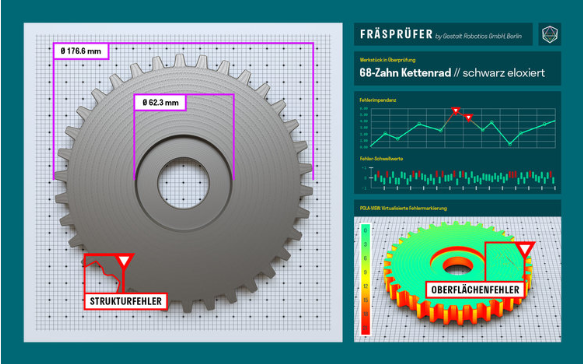
\includegraphics[width=10cm]{images/Gestalt Robotics.png}
  \caption[Qualitätsprüfung-Dashboard von Gestalt Robotics GmbH]{Qualitätsprüfung-Dashboard von Gestalt Robotics GmbH \cite{31}}
\end{figure}

\subsubsection{Digitale Assistenzsyteme}
Das Ziel digitaler Assistenzsysteme ist die Unterstützung der Mitarbeiter beispielsweise durch die Bereitstellung von passenden Informationen, wenn diese benötigt werden. Durch Technologien wie
regelbasierte Planungsalgorithmen und Computer Vision können die Systeme Einsatzsituationen erkennen und Inhalte z.B. angepasst auf das Qualifikationsniveau des Mitarbeiters bereitstellen. Durch maschinelles Lernen können Assistenzsysteme von Nutzer lernen und sich anschließend besser auf ihn einstellen zu können. Mittels Spracherkennung und -generierung können Mensch-Maschine-Schnittstellen bei der Eingabe und Ausgabe von Informationen unterstützt werden.

Eine Anwendung digitaler Assistenzsysteme bietet die Firma TRUMPF GmbH + Co. KG, Hersteller von Laserschneidanlagen und Werkzeugmaschinen. Werden beispielsweise auf einem Blech verschiedene Bauteile ausgeschnitten, erkennt das System welches Bauteil der Mitarbeiter aus dem Blech gelöst hat und zeigt ihm dann den richtigen Ablageort an. \cite{24}

\subsubsection{Prozessoptimierung und -steuerung}
Die Prozesssteuerung beschäftigt sich im Wesentlichen mit der Automatisierung von dynamischen Regelschleifen. Mittels maschinellem Lernens können beispielsweise komplexe Zusammenhänge von verketteten Produktionslinien erkennt werden, die für den Menschen nicht direkt ersichtlich sind.So können z.B. Ursachen für wandernde Engpässe in der Produktion aufgedeckt werden.

Ein Visualisierungs- und Analysewerkzeug von Lana Labs GmbH nutzt welches bereits vorhandene Daten aus beispielsweise einem ERP-System und erstellt darauf basierend automatisiert Prozessmodelle, die einen  Ist-Soll-Zustandsvergleich des Betriebs ermöglicht. Außerdem unterstützt das System bei der Suche nach Ursachen, wenn ein Problem im Prozess auftritt. \cite{24}

\subsubsection{Automatisierungstechnik}
Seit 2011 hat sich der geschätzte Bestand von Industrierobotern weltweit verdreifacht von 1,1 auf knapp 3,5 Millionen Stück.\cite{25} Vor allem in der Automobilindustrie und in der Elektronikbranche sind Industrieroboter im Einsatz. Innerhalb eines Jahres (2018-2019) nahm der Bestand in beiden Branchen jeweils um knapp 80.000 Roboter zu.\cite{26}

Bisher war das Training von Industrierobotern mit hohen Einrichtungskosten bei geringer Flexibilität verbunden. Dadurch lohnten sich diese nur bei häufig wiederholten Prozessen. Doch mittlerweile können Industrieroboter mit Hilfe des maschinellen Lernens neue Prozesse durch das Nachahmen der menschlichen Bewegungen lernen. Bei Übergabepunkten können die Roboter durch Bildverarbeitung die Lage und Orientierung des Bauteils erkennen und entsprechend greifen. Beides erhöht die Flexibilität und Stabilität im Gegensatz zu bisherigen Automatisierungslösungen.
Mit sicherheitszertifizierter Sensorik und Bildverarbeitung ist dann sogar eine  direkte Mensch-Roboter-Kollaboration ohne Sicherheitszaun möglich, die durch Natural Language Processing (NLP)noch intuitiver gestaltet werden.

Die Firma B + M Blumenbecker GmbH ermöglicht mit ihrer KI-Lösung Industrie das Erfassen und Greifen von Bauteilen in beliebiger Lage. Mit Hilfe von Kameras wird die Lage und Orientierung beispielsweise von Schüttgütern in einer Box überwacht, damit das System dann ein Bauteil auswählt, das für den Industrieroboter greifbar ist. Dann wird dieser dort hingeführt. \cite{24}

\chapter{Potenziale für KI in der Produktion}
Technologien der künstlichen Intelligenz finden im letzten Jahrzehnt immer mehr Anwendung in der Wirtschaft und vor allem in der Fertigung. Immer mehr Firmen rüsten ihre Produktion um, um sie effizienter zu gestalten. Wie in Kapitel 2.1 bereits erwähnt, ist das KI-Forschung sehr dynamisch und bringt laufen neue Technologien hervor. Anwendungen für produzierende Unternehmen befinden sich grade noch in den Grundbausteinen, daher werden in den nächsten 5-10 Jahren große Entwicklungsschritte KI in der Produktion erwartet.\cite{08} 
Laut Prognosen von Wissenschaftlern des Instituts für Innovation und Technik soll ein Drittel des Wachstums der produzierenden Industrie in den nächsten fünf auf dem Einsatzes von KI basieren.\cite{24}
Die Erkenntnisse aus der Literaturrecherche  diesem Kapitel wurden im Experteninterview mit Nico Becker, einem Data Scientist und Machine Learning Experten, der über die letzten fünf Jahre zahlreiche Projekte in verschiedenen Branchen als Berater begleitet hat, bestätigt (Protokoll siehe Anhang). Seine Erfahrungen und Einschätzungen aus dem Gebiet der KI und Anwendungen in der Wirtschaft hilft die Potentiale der Technologien zu verstehen.

\section{Hemmnisse zum Einsatz von KI}
In der Literatur und den Fachmedien wird oft das Potenzial von KI-Anwendungen vor allem für produzierende Unternehmen beschrieben. Doch die Umsetzungen in den Unternehmen wird von zahlreichen Faktoren gehemmt. Wie bereits in Kapitel 2.1 beschrieben, sind für die meisten KI-Anwendungen, die über maschinelles Lernen trainiert werden große Datenmengen erforderlich. Da den Unternehmen aber meistens nur eigene Daten zur Verfügung stehen und nur selten ein Datenaustausch zwischen den Fertigungsbetrieben oder auch zwischen den Nutzern und Herstellern von Produktionsmaschinen stattfindet, können KI-Systeme nur mit kleinen Datenmengen trainiert werden. Dies wirkt sich auf die Performance der Anwendungen aus.

Auch die Vielfältigkeit der Produktionen führt zu einem Hemmnis. Da wie im Kapitel 2.2 beschrieben, kaum eine Produktion ist wie die andere, müssen KI-Anwendungen auf die jeweilige Produktion angepasst werden. So können kaum standardisierte, sondern viel mehr individualisierte Lösungen angeboten werden, was zu höheren Kosten führt. Hat ein Unternehmen hierfür kein gut ausgebildetes Personal, kommen Kosten für externe Fachleute hinzu. Dazu kommen Kosten für nötige Modernisierungen bestehender Anlagen oder dem Aufbau neuer Anlagen, um diese Technologien nutzen zu können. Fehlende finanzielle Mittel ist für 80\% der Geschäftsführer von befragten Unternehmen ein Hemmnis zum Einsatz von neuen Technologien der Industrie 4.0. Für Unternehmen ohne Fachpersonal in diesem Bereich ist im allgemeinen schwer die Nutzen solcher Technologien gegen die Kosten abzuwägen. Große Unternehmen können sich solche Anwendungen deshalb eher leisten also mittelständische. Die Komplexität des Themas wird von 58\% der Befragten als Hemmnis wahrgenommen. Ein weiteres Problem, die auch KI-Experte Nico Becker sieht, sind Bedenken und rechtliche Anforderungen bezüglich des Datenschutzes und der Weitergabe sensibler Produktionsdaten. Dies ist ein Hemmnis für mehr als zwei Drittel der Befragten Geschäftsführer, dicht gefolgt von der Anforderung an IT-Sicherheit mit 61\%.\cite{35} Des Weiteren werden auch ethische Themen, die Veränderung der Arbeitswelt und Haftungsfragen als Herausforderungen beim Einsatz von KI in der Produktion in der Literatur diskutiert. Diese werden hier nicht weiter behandelt.

%\section{Bewertungsmethode}
%Technologiemanagement
% Bewertung einsatz KI (Springer-Link)

\section{Potenziale von KI-Anwendungen in der Produktion}

Dass neue Technologien wie KI-Systeme große Potenziale in der Wirtschaft bergen, ist den meisten Unternehmen bewusst. Befragte deutsche Industrieunternehmen sahen 2020 Predictive Maintenance als wichtigsten Vorteil von künstlicher Intelligenz im Kontext von Industrie 4.0, dicht gefolgt von der Steigerung der Produktivität und der Optimierung von Produktions- und Fertigungsprozessen. Als weitere Vorteile werden die bessere Skalierbarkeit und die Reduktion der Kosten gesehen.\cite{28} \newline Auch im Experteninterview mit Nico Becker wird klar, dass KI Technologien in der Produktion eine große Rollen spielen und laufend über weitere mögliche Einsatzszenarien nachgedacht wird. Dennoch schöpfen die wenigsten Unternehmen das volle Potenzial derzeit aus. Vor allem große Unternehmen nutzen bereits KI-Systeme für die Instandhaltung und zur Steigerung der Produktivität, doch oft werden hier nur Lösungen für einzelne Bereiche verwirklicht. Ganzheitliche Konzepte in Zusammenhang mit der Industrie 4.0 sind selten.\cite{02}

Potenziale sind also neben der Entwicklung von neuen KI-Anwendungen die Nutzbarmachung von existierenden und verfügbaren Technologien und dementsprechend der Abbau der im vorhergehen Kapitel beschriebenen Hemmnisse. Betrachtet man die Hürde der hohen Kosten, steckt Potenzial in den Lösungen und Technologien, die einen günstigeren Einsatz von KI ermöglichen. Als Beispiele hierfür nennt Nico Becker AutoML oder Low-Code bzw. No-Code Plattformen, die das Erstellen von KI-Modellen erleichtern. Doch der Einsatz von KI benötigt andere Technologien der Digitalisierung. Durch Edge-Devices, das sind Geräte, die lokal Daten am Rand eines Netzwerkes in Echtzeit verarbeiten, ist es möglich KI-Modelle direkt in Produktionsanlagen einzusetzen, die so ohne eine wesentliche Zeitverzögerung Entscheidungen treffen können. Durch die lokale Erfassung und Verarbeitung großer Datenmengen, werden Speicher- und Übertragungskosten eingespart und nur bestimmte Daten werden in einer Cloud oder andere IT-Infrastruktur übertagen. Hierfür ist eine leistungsstarke Netzwerk-Infrastruktur erforderlich, weshalb hier auch die Industrial 5G Technologie ein wichtige Rolle spielt.\cite{36} Zusammengefasst bedeutet das, dass das Potenzial nicht bei KI alleine liegt, sondern in der Kombination mit anderen Technologien der Digitalisierung.

Vor allem in Deutschland spielt Datenschutz und -sicherheit eine große Rolle. Nur wenige Unternehmen sind bereit sensible Fertigungsdaten an andere Unternehmen weiterzugeben. Doch genau das birgt ein Potenzial. KI-Experte Nico Becker gibt folgendes Beispiel: Stellt ein produzierendes Unternehmen als Nutzer einer Maschine dem Hersteller Sensordaten zur Verfügung, die während der Nutzung der Maschine erfasst werden, kann dieser Verbesserungen an der Maschine vornehmen und detailliertere Informationen über den Zustand bereit stellen.\newline
Allgemein nutzen Unternehmen ihre Daten kaum. So werden weniger als ein Prozent der unstrukturierten Daten analysiert, wobei der Anteil dieser "Dark Data" bei bis 80\% der generierten Daten liegt.\cite{36}

Im vorherigen Kapitel wurde auch die hohe Komplexität als Hürde beschrieben. Aus diesem Grund sieht Nico Becker im Experteninterview das Thema Computer Vision als Potenzial, da gerade die Methode für den Menschen gut nachvollziehbar und intuitiv. So nutzen auch menschliche Prüfer ''das Sehen'', um zu urteilen und zu entscheiden. Zwar gibt es schon zahlreiche Anwendungen mit dieser KI-Technologie, doch das Potenzial ist hier noch nicht ausgeschöpft. \newline Auch andere Anwendungen, die dem Nutzer visuelle Informationen aufbereiten werden in der Literatur als vielversprechende Technologien gesehen, wie z.B. Extended Reality. Unter diesem Ausdruck sind Augmented(AR), Mixed (MR) und Virtual Reality (VR) zusammengefasst. Die Technologien werden vor allem im Zusammenhang mit digitalen Assistenzsystemen verwendet. Um eine intuitive Interaktion zwischen dem Nutzer und dem System zu ermöglichen werden KI-Technologien, wie Spracherkennung und -generierung verwendet. Dies ermöglicht einer bessere Reaktionsfähigkeit des Systems auf den Nutzer und präziseres Feedback. Diese Technologien kommen bereits zum Einlernen und Trainieren von Mitarbeitenden zum Einsatz, wobei trotzdem Bildschirme oder Tablets nach wie vor am häufigsten verwendet werden.\cite{37} \newline
Ein weitere Ansatz, der die Komplexität der Technologien mindern könnte, sind technisch besser qualifizierte Mitarbeiter. Trotz Digitalisierung wird der Mensch weiterhin unverzichtbar in einer Produktion sein. Zwar übernehmen Maschinen immer mehr standardisierte Aufgaben, doch für Problemfälle, planerische und konzeptionelle Aufgaben und Lösungen wird menschliche Intelligenz und Kreativität benötigt. So sinkt der Anteil manueller Tätigkeiten, doch der Bedarf an IT-Verständnis steigt.\cite{36} Mit Hilfe von technisch gut ausgebildetem Personal, das sich schneller auf neue Technologien einstellen kann, sinkt die Hürde der Komplexität. Denn die Literatur ist sich einige, der Mensch wird weiterhin eine wichtige Rolle in produzierenden Unternehmen spielen. Das Ziel ist es das Arbeiten von KI und Mensch nebeneinader umzuwandeln, sodass die KI die Arbeit der Menschen vereinfacht und bereichert.\cite{02}

Neben diesen Potenzialen, bieten Lösungen der Digitalisierung und KI auch eine Möglichkeit die Produktion nachhaltiger zu gestalten. Durch diese Technologien Ressourcen wie Energie, Wasser und Abwasser gespart werden und Abfall, sowie CO2-Emissionen reduziert werden. \cite{36}\newline
Eine vielversprechende Technologie, die in Bezug auf Digitalisierung und KI in der Produktion oft genannt wird, ist der sogenannte ''Digitale Zwilling (DZ)''. Er stellt eine virtuelle Abbildung eines physischen Gegenstücks dar, z.B. eines Produktes, Prozesses, einer Produktionsanlage oder sogar einer ganzen Fabrik dar. Beide sind über konstantes Datenaustausch miteinander verbunden. So sind Informationen über das reale Objekt auch sofort digital zugänglich und können weiterverarbeitet werden. Auch andersherum kann durch Änderungen am virtuellen Objekt, das reale Gegenstück beeinflusst werden. Für die meisten Anwendungen des DZ werden maschinelles Lernen, Bild- und Tonverarbeitung, Mustererkennung und weitere KI-Technologien genutzt.
Neu ist das Konzept eines digitalen Zwillings nicht. Schon 2012 stellte die NASA den digitalen Zwilling als zukunftsweidende Technologie für die Entwicklung und Simulation für Luft- und Raumfahrt dar. Auch in der Produktionswirtschaft hat diese Technologie großes Potenzial, denn es kann für zahlreiche Anwendungen, wie unter anderem Prognosen, Analysen und zur Prozessoptimierung genutzt werden.\cite{32}

\begin{figure}[H]
  \center
 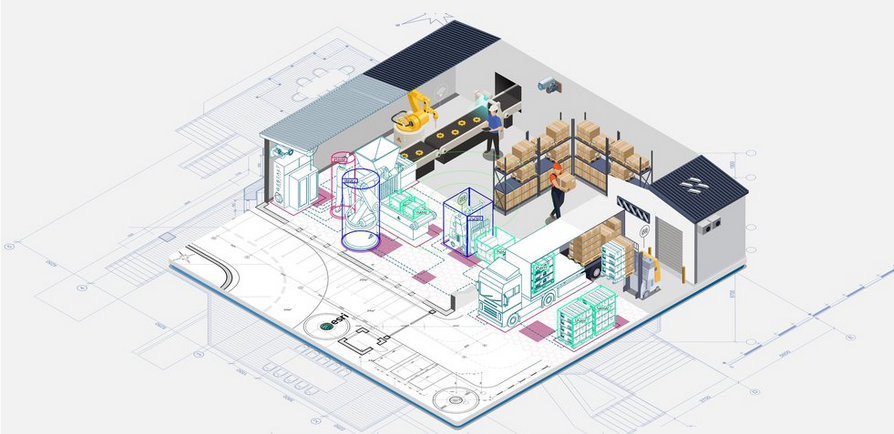
\includegraphics[width=10cm]{images/DZ.png}
  \caption[Digitaler Zwilling in Produktion und Logistik]{Digitaler Zwilling in Produktion und Logistik \cite{34}}
\end{figure}

Trotz dessen, dass die Technologie des digitalen Zwillings schon in zahlreichen produzierenden Unternehmen für unterschiedlichste Anwendungsbereiche genutzt wird, ist sie hier als Potenzial aufgeführt. Denn durch die zunehmend digitalisierten Produktionen und nutzbaren Daten sind immer mehr Anwendungen möglich. Die Möglichkeiten werden teilweise als nahezu grenzenlos beschrieben, da die meisten bisherigen Anwendungen von KI in der Produktion darin vereint werden können. Neben der Instandhaltung und der Steuerung und Überwachung der Produktionsmaschinen, können auch Prozesse beliebig über die gesamte Wertschöpfungskette simuliert werden. Daraus entsteht ein großes Potential zur Steigerung der Flexibilität, Effizienz, Qualität, Effektivität, aber auch zur Senkung der Kosten und Komplexität von Prozessen und Minderung des Risikos bei Veränderungen.\cite{33}

Nicht nur klassische produzierende Unternehmen aus dem Maschinenbau, der Automobil- oder Elektronikindustrie können von KI-Technologien profitieren, auch die Produktion von kulturellen Gütern, wie Bilder, Texte, Ton- und Musikaufnahmen und Bewegtbilder kann dieses Potenzial nutzen. Schon aktuell können beispielsweise Bilder nur durch Eingabe von Vorgaben von einer KI wie DALL.E 2 von OpenAI oder Stable Diffusion von Hugging Face generiert werden. Dies ist auch mit Videos möglich, wie Unternehmen wir MetaAI mit Make-a-video beweisen. Zwar sind diese generierten Bilder und Videos derzeit noch eine lustige Spielerei mit nicht allzu hoher Qualität, doch in Zukunft könnten derartige KI-Systeme für die Filmindustrie von Nutzen sein. Special Effects und Filmsets könnten so anstatt aufwendig animiert und gebaut zu werden, durch eine KI generiert werden.

\begin{figure}[H]
  \center
 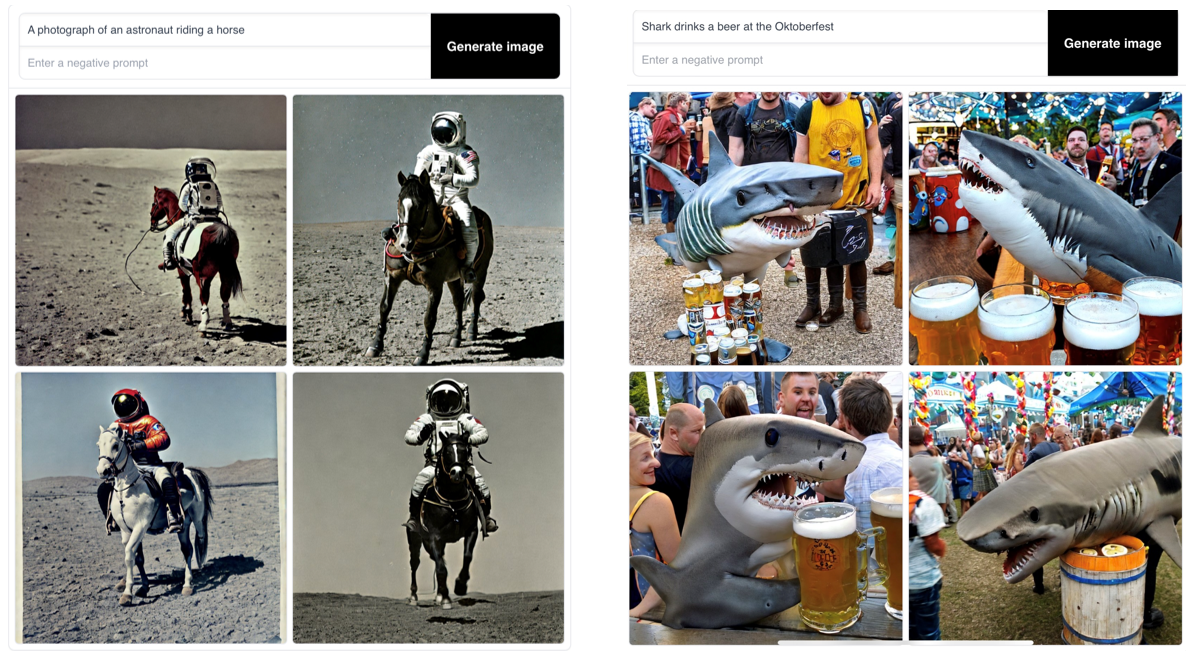
\includegraphics[width=14cm]{images/stableDif.png}
  \caption[Bilder generiert von Stable Diffusion]{Bilder generiert von Stable Diffusion \cite{38}}
\end{figure}

Innerhalb von Europa gibt es Initiativen und Forschungsprojekte, die sich mit Potenzialen in der Produktion beschäftigen, z.B. EuProGigant vom Österreichisch-Deutschem Projektkonsortium. Deren Ziel ist es zentrale Fragestellungen zum Thema ''Smarte und souveräne Nutzung von Daten für die Produktion'' zu bearbeiten. Damit wollen sie unter anderem Ziele, wie eine Produktivitätssteigerung von 10\% erreichen.\cite{39}
\begin{figure}[H]
  \center
 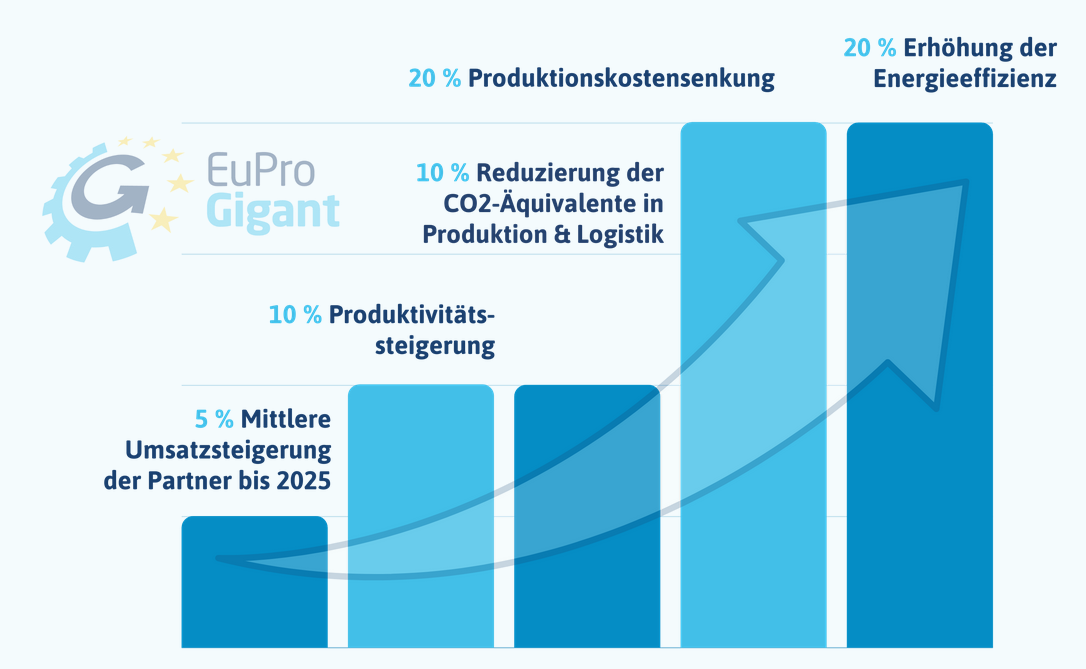
\includegraphics[width=10cm]{images/eupro.png}
  \caption[Zielwirkung von EuProGigant]{Zielwirkung von EuProGigant \cite{39}}
\end{figure}

Im internationalen Vergleich steht Deutschland im Bezug auf die digitale Transformation gut da. Damit das auch weiterhin der Fall ist, müssen Politik, Wirtschaft, Wissenschaft und Gesellschaft weiterhin einigen Hürden stellen. Beispiele sind der Ausbau einer flächendeckende und schnelle Datenübertragung, neue Bildungskonzepte und reicht bis zu einem Mentalitätswandel von Wirtschaft und Gesellschaft. \cite{36}

\chapter{Fazit und Ausblick}

Sowohl der Forschungsbereich der künstlichen Intelligenz als auch die KI-Anwendungen, die für die Produktion genutzt werden können, entwickeln sich stetig und schnell weiter. Die Vorteile und Potenziale, die solche Technologien bieten, sind in der Industrie bekannt. Trotzdem sind viele vor allem kleine Unternehmen eher zurückhaltend, was die Implementierung dieser Lösungen angeht. Für sie ist es schwer abzuschätzen, ob der Nutzen die Kosten aufwiegt. Auch andere Hausforderungen, wie das Black-Box-Verhalten von Technologien mit maschinellem Lernen, die hohen Kosten zur Implementierung von KI-Technologien und Datensicherheit wirken hemmend. Trotzdem zeigen Vorreiter der produzierenden Industrie, dass sich der Einsatz smarter Lösungen lohnt. Die Potenziale für Technologien der künstlichen Intelligenz in der Produktion sind groß und werden sich in den nächsten Jahren auch Grund des technischen Fortschritts immer weiter vergrößern. Doch auch die Nutzbarmachung der bereits vorhandenen Technologien ist wichtig.\newline
Klar ist, dass das Potenzial nicht alleine bei KI liegt, sondern Themen aus der Digitalisierung und der Datenverarbeitung eine mindestens genauso große Rollen dabei spielen Produktionen effizienter zu gestalten.

\listoffigures

\clearpage




\clearpage
\addcontentsline{toc}{chapter}{Literaturverzeichnis}

% Nochmal recherchieren wie man IEEE Standard im Literaturverzeichnis umsetzt


\begin{thebibliography}{99}

\bibitem{01}
	P. Buxmann, H. Schmidt,
	Künstliche Intelligenz: Mit Algorithmen zum wirtschaftlichen Erfolg,
	Springer Gabler,
	2.Auflage,
	2021.
	
\bibitem{02}
	A. Mockenhaupt,
	Digitalisierung und Künstliche Intelligenz in der Produktion: Grundlagen und Anwendung,
	Springer Vieweg,
	2021.

\bibitem{03}
	T. Kaufmann, H. Servatius,
	Das Internet der Dinge und Künstliche Intelligenz als Game Changer: Wege zu einem Management 4.0 und einer digitalen Architektur,
	Springer Vieweg,
	2020.

\bibitem{04} 	
	ChatGPT,
	OpenAI,
	Aufgerufen am 14.01.2023.

\bibitem{05}
	C. Appugliese, P. Nathan, W. S. Roberts
	Agil AI
	O´Reilly Media, Inc.,
	2020.

\bibitem{06}
	GI. Spindler,
	Produktion in Basiswissen Allgemeine Betriebswirtschaftslehre,
	p. 27-46,
	Springer Gabler,
	2022.

\bibitem{07}
	J. Bloech, R. Bogaschewsky, U. Buscher, A. Daub, U. Götze, F. Roland,
	Einführung in die Produktion,
	Springer Gabler, 
	2014.
	
\bibitem{08}
	I. Knappertsbusch, K. Gondlach,
	Arbeitswelt und KI 2030: Herausforderungen und Strategien für die Arbeit von morgen,
	Springer Gabler,
	2022.

\bibitem{09}
	R. Buchkremer, T. Heupel, O. Koch,
	Künstliche Intelligenz in Wirtschaft \& Gesellschaft: Auswirkungen, Herausforderungen \& Handlungsempfehlungen
	Springer Gabler,
	2020.

\bibitem{10}
	C. Welzel, D. Grosch,
	Das ÖFIT-Trendsonar Künstliche Intelligenz,
	Kompetenzzentrum Öffentliche Informationstechnologie,
	2018.

\bibitem{11}
	W. Ertel,
	Grundkurs Künstliche Intelligenz: Eine praxisorientierte Einführung,
	5. Auflage,
	Springer Vieweg,
	2021.

\bibitem{12}
	H. J. Wildermann, K. J. Schmidt,
	Produktion, 
	in: W. Lück, Lexikon der Betriebswirtschaft,
	Verlag moderne Industrie,
	1990.


\bibitem{15}
	T. Zwingmann,
	AI-Powered Business Intelligence,
	O'Reilly Media, Inc.,
	2022.

\bibitem{16}
	U.Walter,
	Künstliche Intelligenz für Dummies (Vortrag),
	Deutsches Museum München,
	https://www.youtube.com/watch?v=B7vCtHvYMyE
	2020.

\bibitem{17}
	D. Sonnet,
	Neuronale Netze kompakt: Vom Perceptron zum Deep Learning,
	Springer Vieweg,
	2022.

\bibitem{18}
	C. Steger, M. Ulrich, C. Wiedemann,
	Machine Vision Algorithms and Applications,
	Wiley-VCH,
	2018.

\bibitem{19}
	A. Jorzig, F. Sarangi,
	Künstliche Intelligenz und Robotik, 
	in: Digitalisierung im Gesundheitswesen,
	Springer,
	2020.

\bibitem{20}
	E. Gutenberg,
	Grundlagen der Betriebswirtschaftslehre, Band 1: Produktion,
	Springer,
	1951.




\end{thebibliography}

\appendix
\section{Abbildungen}



\section{Experteninterview}


\end{document}